%%%%%%%%%%%%%%%%%%%%%%%%%%%%%%%%%%%%%%%%%
% Beamer Presentation
% LaTeX Template
% Version 1.0 (10/11/12)
%
% This template has been downloaded from:
% http://www.LaTeXTemplates.com
%
% License:
% CC BY-NC-SA 3.0 (http://creativecommons.org/licenses/by-nc-sa/3.0/)
%
%%%%%%%%%%%%%%%%%%%%%%%%%%%%%%%%%%%%%%%%%

%----------------------------------------------------------------------------------------
%	PACKAGES AND THEMES
%----------------------------------------------------------------------------------------

\documentclass{beamer}

\mode<presentation> {

% The Beamer class comes with a number of default slide themes
% which change the colors and layouts of slides. Below this is a list
% of all the themes, uncomment each in turn to see what they look like.

%\usetheme{default}
%\usetheme{AnnArbor}
%\usetheme{Antibes}
%\usetheme{Bergen}
%\usetheme{Berkeley}
%\usetheme{Berlin}
%\usetheme{Boadilla}
%\usetheme{CambridgeUS}
%\usetheme{Copenhagen}
%\usetheme{Darmstadt}
%\usetheme{Dresden}
%\usetheme{Frankfurt}
%\usetheme{Goettingen}
%\usetheme{Hannover}
%\usetheme{Ilmenau}
%\usetheme{JuanLesPins}
%\usetheme{Luebeck}
\usetheme{Madrid}
%\usetheme{Malmoe}
%\usetheme{Marburg}
%\usetheme{Montpellier}
%\usetheme{PaloAlto}
%\usetheme{Pittsburgh}
%\usetheme{Rochester}
%\usetheme{Singapore}
%\usetheme{Szeged}
%\usetheme{Warsaw}

% As well as themes, the Beamer class has a number of color themes
% for any slide theme. Uncomment each of these in turn to see how it
% changes the colors of your current slide theme.

%\usecolortheme{albatross}
%\usecolortheme{beaver}
%\usecolortheme{beetle}
%\usecolortheme{crane}
%\usecolortheme{dolphin}
%\usecolortheme{dove}
%\usecolortheme{fly}
%\usecolortheme{lily}
%\usecolortheme{orchid}
%\usecolortheme{rose}
%\usecolortheme{seagull}
%\usecolortheme{seahorse}
\usecolortheme{whale}
%\usecolortheme{wolverine}

\setbeamertemplate{footline} % To remove the footer line in all slides uncomment this line
%\setbeamertemplate{footline}[page number] % To replace the footer line in all slides with a simple slide count uncomment this line

\setbeamertemplate{navigation symbols}{} % To remove the navigation symbols from the bottom of all slides uncomment this line

}

\usepackage{graphicx} % Allows including images
\usepackage{booktabs} % Allows the use of \toprule, \midrule and \bottomrule in tables
\usepackage{sansmathaccent}
\pdfmapfile{+sansmathaccent.map}

\usepackage{tikz}
\usetikzlibrary{trees, shapes, shapes.geometric, decorations, arrows, positioning}

%----------------------------------------------------------------------------------------
%	TITLE PAGE
%----------------------------------------------------------------------------------------

\title[Short title]{Balanced Trees} % The short title appears at the bottom of every slide, the full title is only on the title page

%\author{John Smith} % Your name
\institute[BYU] % Your institution as it will appear on the bottom of every slide, may be shorthand to save space
{
Brigham Young University \\ % Your institution for the title page
\medskip
%\textit{john@smith.com} % Your email address
}
\date{\today} % Date, can be changed to a custom date

\begin{document}

\tikzset{
    bnode/.style = {   
        text width=1.0em, align=center,                                           
        draw,
        rectangle split,
        rectangle split horizontal,
        rectangle split parts=4,
        rectangle split draw splits=true
    }
}
\begin{frame}
\titlepage % Print the title page as the first slide
\end{frame}

%\begin{frame}
%\frametitle{Overview} % Table of contents slide, comment this block out to remove it
%\tableofcontents % Throughout your presentation, if you choose to use \section{} and %\subsection{} commands, these will automatically be printed on this slide as an overview of your presentation
%\end{frame}

%----------------------------------------------------------------------------------------
%	PRESENTATION SLIDES
%----------------------------------------------------------------------------------------

%------------------------------------------------
%\section{First Section} % Sections can be created in order to organize your presentation into %discrete blocks, all sections and subsections are automatically printed in the table of contents %as an overview of the talk
%------------------------------------------------

%\subsection{Subsection Example} % A subsection can be created just before a set of slides with %a common theme to further break down your presentation into chunks

%\begin{frame}
%\frametitle{AVL trees}
%Sed iaculis dapibus gravida. Morbi sed tortor erat, nec interdum arcu. Sed id lorem lectus. %Quisque viverra augue id sem ornare non aliquam nibh tristique. Aenean in ligula nisl. Nulla sed %tellus ipsum. Donec vestibulum ligula non lorem vulputate fermentum accumsan neque mollis.%\\~\\

%Sed diam enim, sagittis nec condimentum sit amet, ullamcorper sit amet libero. Aliquam vel dui %orci, a porta odio. Nullam id suscipit ipsum. Aenean lobortis commodo sem, ut commodo leo %gravida vitae. Pellentesque vehicula ante iaculis arcu pretium rutrum eget sit amet purus. %Integer ornare nulla quis neque ultrices lobortis. Vestibulum ultrices tincidunt libero, quis %commodo erat ullamcorper id.
%\end{frame}

%------------------------------------------------

\begin{frame}
\frametitle{Trees}
\begin{center}

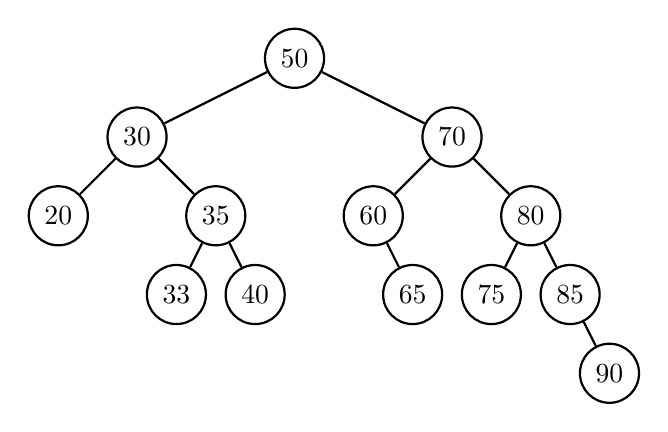
\begin{tikzpicture}[
  level distance=1 cm, % Normally, this distance would be 1.5cm, but the original pictures to imitate are more condensed
  level 1/.style={sibling distance=4cm}, % Adjust the level distance to compensate for additional nodes
  level 2/.style={sibling distance=2cm},
  level 3/.style={sibling distance=1cm},
   thick, minimum size = .75cm]

  \node[circle,draw] {50}
	child {node[circle,draw]{30}
		child{node[circle,draw]{20}}
		child{node[circle,draw]{35}
			child{node[circle,draw]{33}}
			child{node[circle,draw]{40}}
		}
	}
	child{node[circle,draw]{70}
		child{node[circle,draw]{60}
			child[fill=none] {edge from parent[draw=none]} 
			child{node[circle,draw]{65}}
		}
		child{node[circle,draw]{80}
			child{node[circle,draw]{75}}
			child{node[circle,draw]{85}
				child[fill=none] {edge from parent[draw=none]} 
				child{node[circle,draw]{90}}	
			}
		}
	};
\end{tikzpicture}

\end{center}
\begin{itemize}
\item Worst case complexity is $O(\log n)$ for inserting, deleting, and searching.
\end{itemize}
\end{frame}

%------------------------------------------------
\begin{frame}
\frametitle{Binary Search Tree}
\begin{itemize}
\item The \textbf{Binary Search Tree} or BST is the most basic tree based data structure.
\item Each node or vertex has two children - left and right.
\item This gives the tree an order:
	\begin{itemize}
	\item Everything in the left subtree is less than the node.
	\item Everything in the right subtree is greater.
	\end{itemize}
\item Searching is efficient. Start at the root of the tree and step to the left or right each time.
\item This cuts out half of the tree at each step, making search time $O(\log n)$.
\end{itemize}
\end{frame}

%------------------------------------------------
\begin{frame}
\frametitle{Binary Seach Tree Problems}
\begin{itemize}
\item Adding already sorted or nearly sorted data to a binary search tree essential results in a linked list.
\item BSTs are best for inserting random data.
\item The more levels a tree has, the less performant it becomes. 
\item Filling each level can minimize the number of levels a BST has.
\end{itemize}
\end{frame}
%----------------------------------------------
\begin{frame}
\frametitle{BST}
Adding ordered data leads to the left tree.
Balancing gives the right tree.
To find $99$ search 7 levels or 3.
\begin{columns}[c]
\column{.5\textwidth}
\begin{center}

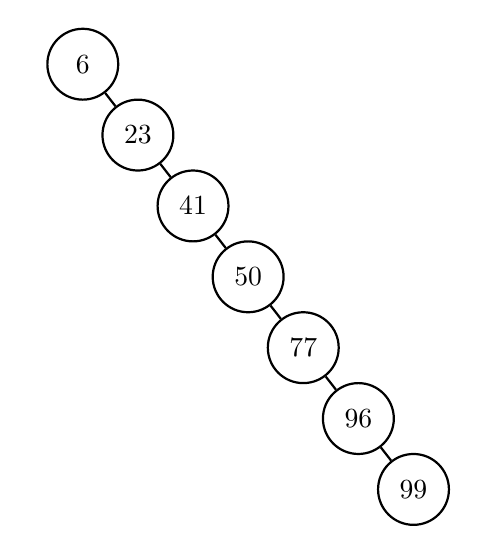
\begin{tikzpicture}[
  level distance=.9 cm,
  sibling distance=1.4cm,
  thick, minimum size = .9cm] % level distance shortened to prevent taking up too much space on the page

  \node[circle,draw] {6}
	child[fill=none] {edge from parent[draw=none]}	
	child {node[circle,draw]{23}
		child[fill=none] {edge from parent[draw=none]}
		child{node[circle,draw]{41}
			child[fill=none] {edge from parent[draw=none]}
			child{node[circle,draw]{50}
				child[fill=none] {edge from parent[draw=none]}
				child{node[circle,draw]{77}
					child[fill=none] {edge from parent[draw=none]}
					child{node[circle,draw]{96}
						child[fill=none] {edge from parent[draw=none]}
						child{node[circle,draw]{99}}
					}
				}
			}
		}
	};
\end{tikzpicture}

\end{center}
\column{.5\textwidth}
\begin{center}

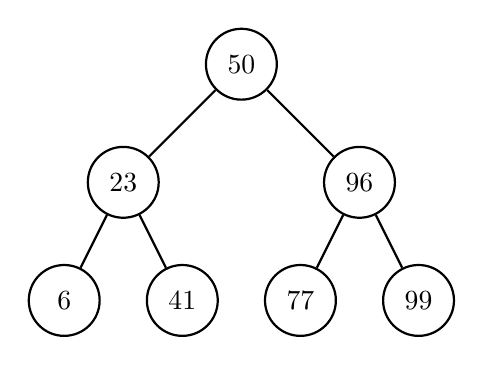
\begin{tikzpicture}[
  level distance=1.5 cm,
  level 1/.style={sibling distance=3cm},
  level 2/.style={sibling distance=1.5cm},
 thick, minimum size = .9cm]

  \node[circle,draw] {50}
	child {node[circle,draw]{23}
		child{node[circle,draw]{6}
		}
		child{node[circle,draw]{41}
		}
	}
	child{node[circle,draw]{96}
		child{node[circle,draw]{77}
		}
		child{node[circle,draw]{99}
		}
	};
\end{tikzpicture}

\end{center}

\end{columns}



\end{frame}

%------------------------------------------------
\begin{frame}
\frametitle{AVL trees}
\begin{itemize}
\item \textbf{AVL Trees} are balanced BSTs.
\item AVL trees determine balance by comparing the height of the right and left subtrees.
\item The height of a node is the length from that node to its deepest leaf node.
\item Or the maximum of the heights of the two subtrees plus one.

\end{itemize}
\end{frame}
%------------------------------------------------
\begin{frame}
\frametitle{AVL Trees}
\begin{columns}[c]
\column{.4\textwidth}
\begin{itemize}
\only<1>{
\item For every node in an AVL tree, if the difference of heights between the left and right subtrees is more than $\pm 1$ level, then the tree is \emph{out of balance}.
\item Restore balance to the entire tree by rearranging the subtrees.
}
\only<2>{
\item This tree is balanced, because the difference in heights of neighboring subtrees is never more than 1.
}
\end{itemize}
\column{.6\textwidth}
\begin{center}

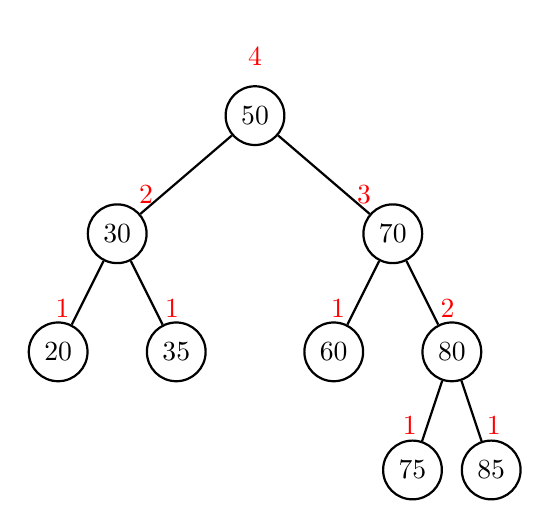
\begin{tikzpicture}[
  level distance=1.5 cm, % Normally, this distance would be 1.5cm, but the original pictures to imitate are more condensed
  level 1/.style={sibling distance=3.5cm}, % Adjust the level distance to compensate for additional nodes
  level 2/.style={sibling distance=1.5cm},
  level 3/.style={sibling distance=1cm},
   thick]

  \node[circle,draw] (50){50}
	child {node[circle,draw]{30}
		child{node[circle,draw]{20}
			edge from parent node[near end, left, red]{1}}
		child{node[circle,draw]{35}
			edge from parent node[near end, right, red]{1}}
		edge from parent node[near end, left, red]{2}
	}
	child{node[circle,draw]{70}
		child{node[circle,draw]{60}
			edge from parent node[near end, left, red]{1}
		}
		child{node[circle,draw]{80}
			child{node[circle,draw]{75}
				edge from parent node[near end, left, red]{1}}
			child{node[circle,draw]{85}
				edge from parent node[near end, right, red]{1}}
			edge from parent node[near end, right, red]{2}
		}
		edge from parent node[near end, right, red]{3}
	};
     \node[draw=none, node distance=1cm](4)[above of=50]{};
   \draw[] (4) edge[draw=none, near start, red] node {4} (50);
\end{tikzpicture}

\end{center}

\end{columns}
\end{frame}

%------------------------------------------------

\begin{frame}
\frametitle{Left-Left and Right-Right}
%TODO: nicer triangles
\begin{columns}[c] 

\column{.35\textwidth}
\begin{itemize}
\only<1>{
\item The top is a Left-Left case
  \begin{itemize}
  \item C's left subtree is greater than C's right subtree
  \item B's left subtree is greater than B's right subtree
  \end{itemize}
  }
\only<2>{
\item The Right-Right case is the mirror opposite.
\item Need one rotation.}
\end{itemize}
\column{.65\textwidth}
\begin{center}

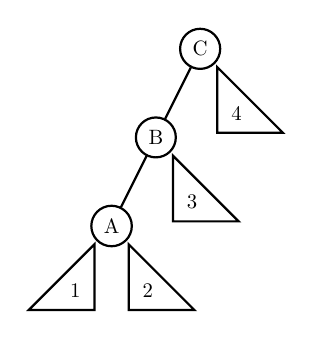
\begin{tikzpicture}[scale=.75, transform shape,
  level distance=1.5 cm,
  level 1/.style={sibling distance=1.5cm},
  level 2/.style={sibling distance=1.5cm},
  thick]

  \node[circle,draw] (C){C}
	child {node[circle,draw](B){B}
		child {node[circle,draw](A){A}}
		child[fill=none] {edge from parent[draw=none]}
		}
	child[fill=none] {edge from parent[draw=none]};


    \node[draw, shape border uses incircle, isosceles triangle,isosceles triangle apex angle=90, shape border rotate=-45](1)[below left of=A, anchor=north, node distance=0.87cm]{1};
    \node[isosceles triangle, draw, shape border uses incircle, isosceles triangle,isosceles triangle apex angle=90, shape border rotate=225](4)[below right of=A, anchor=north, node distance=0.87cm]{2};
  \node[isosceles triangle, draw, shape border uses incircle, isosceles triangle,isosceles triangle apex angle=90, shape border rotate=225](4)[below right of=B, anchor=north, node distance=0.87cm]{3};
  \node[isosceles triangle, draw, shape border uses incircle, isosceles triangle,isosceles triangle apex angle=90, shape border rotate=225](4)[below right of=C, anchor=north, node distance=0.87cm]{4};
\end{tikzpicture}

\vspace{.5cm}

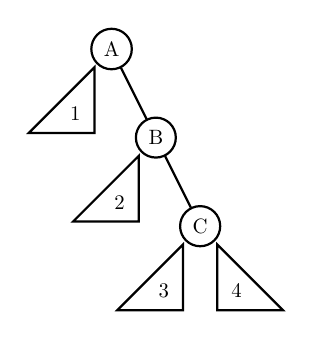
\begin{tikzpicture}[scale=.75, transform shape,
  level distance=1.5 cm,
  level 1/.style={sibling distance=1.5cm},
  level 2/.style={sibling distance=1.5cm},
  thick]

  \node[circle,draw] (A){A}
	child[fill=none] {edge from parent[draw=none]}
	child {node[circle,draw](B){B}
		child[fill=none] {edge from parent[draw=none]}		
		child {node[circle,draw](C){C}}
		};


  \node[draw, shape border uses incircle, isosceles triangle,isosceles triangle apex angle=90, shape border rotate=-45][below left of=A, anchor=north, node distance=0.87cm]{1};
  \node[draw, shape border uses incircle, isosceles triangle,isosceles triangle apex angle=90, shape border rotate=-45][below left of=B, anchor=north, node distance=0.87cm]{2};
  \node[draw, shape border uses incircle, isosceles triangle,isosceles triangle apex angle=90, shape border rotate=-45][below left of=C, anchor=north, node distance=0.87cm]{3};
  \node[isosceles triangle, draw, shape border uses incircle, isosceles triangle,isosceles triangle apex angle=90, shape border rotate=225][below right of=C, anchor=north, node distance=0.87cm]{4};
\end{tikzpicture}
\end{center}
\end{columns}
\end{frame}

%------------------------------------------------

\begin{frame}
\frametitle{Left-Left and Right-Right}
\begin{columns}[c] 
\column{.35\textwidth}
\begin{itemize}
\item Rotate the nodes so that B is the new root of the tree.
\item C becomes a right child of B and the right subtree of B becomes a left subtree of C.
\item This preserves the ordered property of the tree.
\end{itemize}
\column{.5\textwidth}
\begin{center}
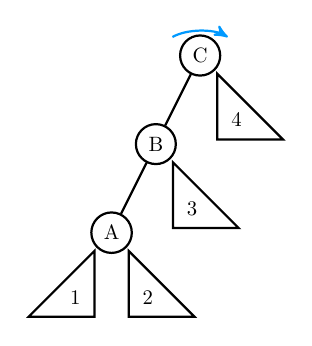
\begin{tikzpicture}[scale=.75, transform shape,
  node distance = .7cm,
  level distance=1.5 cm,
  level 1/.style={sibling distance=1.5cm},
  level 2/.style={sibling distance=1.5cm},
  thick]

  \node[circle,draw] (C){C}
	child {node[circle,draw](B){B}
		child {node[circle,draw](A){A}}
		child[fill=none] {edge from parent[draw=none]}
		}
	child[fill=none] {edge from parent[draw=none]};


    \node[draw, shape border uses incircle, isosceles triangle,isosceles triangle apex angle=90, shape border rotate=-45](1)[below left of=A, anchor=north, node distance=0.87cm]{1};
    \node[isosceles triangle, draw, shape border uses incircle, isosceles triangle,isosceles triangle apex angle=90, shape border rotate=225](4)[below right of=A, anchor=north, node distance=0.87cm]{2};
  \node[isosceles triangle, draw, shape border uses incircle, isosceles triangle,isosceles triangle apex angle=90, shape border rotate=225](4)[below right of=B, anchor=north, node distance=0.87cm]{3};
  \node[isosceles triangle, draw, shape border uses incircle, isosceles triangle,isosceles triangle apex angle=90, shape border rotate=225](4)[below right of=C, anchor=north, node distance=0.87cm]{4};
  
    \node[circle, draw=none] [left of=C](L){};
  \node[circle, draw=none] [right of=C](R){};
    \path[->, >=stealth', auto]
      (L.north) edge[bend left, shorten >=.2cm, shorten <=.2cm, blue!40!cyan ] (R.north);
\end{tikzpicture}

\vspace{.5cm}

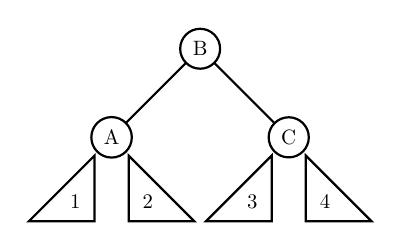
\begin{tikzpicture}[scale=.75, transform shape,
  level distance=1.5 cm,
  level 1/.style={sibling distance=3cm},
  level 2/.style={sibling distance=1.5cm},
  thick]

  \node[circle,draw] (B){B}
	child {node[circle,draw](A){A}}
	child {node[circle,draw](C){C}};
	
  \node[draw, shape border uses incircle, isosceles triangle,isosceles triangle apex angle=90, shape border rotate=-45](1)[below left of=A, anchor=north, node distance=0.87cm]{1};
    \node[isosceles triangle, draw, shape border uses incircle, isosceles triangle,isosceles triangle apex angle=90, shape border rotate=225](4)[below right of=A, anchor=north, node distance=0.87cm]{2};
  \node[draw, shape border uses incircle, isosceles triangle,isosceles triangle apex angle=90, shape border rotate=-45](2)[below left of=C, anchor=north, node distance=0.87cm]{3};
  \node[isosceles triangle, draw, shape border uses incircle, isosceles triangle,isosceles triangle apex angle=90, shape border rotate=225](4)[below right of=C, anchor=north, node distance=0.87cm]{4};
\end{tikzpicture}

\end{center}
\end{columns}

\end{frame}


%------------------------------------------------
\begin{frame}
\frametitle{Balance}

\begin{columns}[c]
\column{.5\textwidth}
\begin{itemize}

\item The Left subtree is out of balance.
  \begin{itemize}
  \item 5 has a height of 3
  \item 15 has a hieght of 1.
  \end{itemize}
\item Right-Right case 
  \begin{itemize}
  \item 5's right subtree is heaveir than the left 
  \item 7's right subtree is heavier than the left.
  \end{itemize}
\end{itemize}

\column{.5\textwidth}
\begin{center}
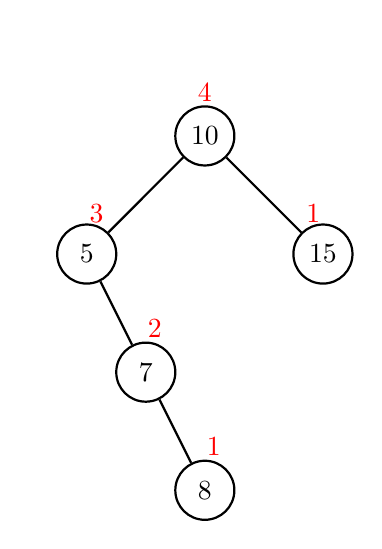
\begin{tikzpicture}[
  level distance=1.5 cm,
  level 1/.style={sibling distance=3cm},
  level 2/.style={sibling distance=1.5cm},
  level 3/.style={sibling distance=1.5cm},
  minimum size=.75cm, thick]

  \node[circle,draw] (10){10}
	child {node[circle,draw]{5}
		child[fill=none] {edge from parent[draw=none]}
		child{node[circle,draw]{7}
			child[fill=none] {edge from parent[draw=none]}
			child{node[circle,draw]{8}
				edge from parent node[near end, right, red]{1}}
			edge from parent node[near end, right, red]{2}
		}
		edge from parent node[near end, left, red]{3}
	}
	child{node[circle,draw]{15}
		edge from parent node[near end, right, red]{1}
	};
     \node[draw=none, node distance=1cm](4)[above of=10]{};
   \draw[] (4) edge[draw=none, near start, red] node {4} (10);
\end{tikzpicture}
\end{center}
\end{columns}
\end{frame}

%--------------------------------------------------
\begin{frame}
\frametitle{Balance the Tree}
\begin{columns}[c]
\column{.5\textwidth}
\begin{itemize}
\item Rotate left on 5.
\end{itemize}

\column{.5\textwidth}
\begin{center}
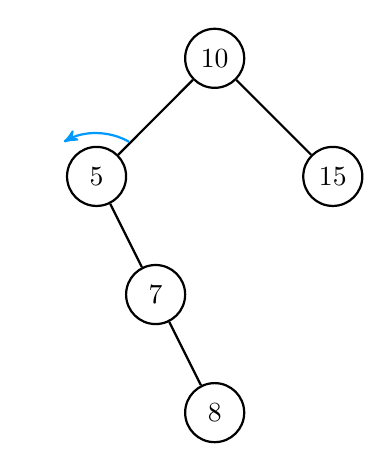
\begin{tikzpicture}[
  level distance=1.5 cm,
  node distance = .5cm,
  level 1/.style={sibling distance=3cm},
  level 2/.style={sibling distance=1.5cm},
  level 3/.style={sibling distance=1.5cm},
  minimum size=.75cm, thick]

  \node[circle,draw] {10}
	child {node[circle,draw](5){5}
		child[fill=none] {edge from parent[draw=none]}
		child{node[circle,draw]{7}
			child[fill=none] {edge from parent[draw=none]}
			child{node[circle,draw]{8}}
		}
	}
	child{node[circle,draw]{15}
	};
  \node[circle, draw=none] [left of=5](L){};
  \node[circle, draw=none] [right of=5](R){};
    \path[->, >=stealth', auto]
      (R.north) edge[bend right, shorten >=.1cm, shorten <=.1cm, blue!40!cyan ] (L.north);
\end{tikzpicture}
\end{center}
\end{columns}

\end{frame}

%-----------------------------------------------
\begin{frame}
\frametitle{Balance the Tree}
\begin{columns}[c]
\column{.5\textwidth}
\begin{itemize}
\item7 becomes the root of the subtree
\item 5 becomes 7's left child.
\end{itemize}

\column{.5\textwidth}
\begin{center}

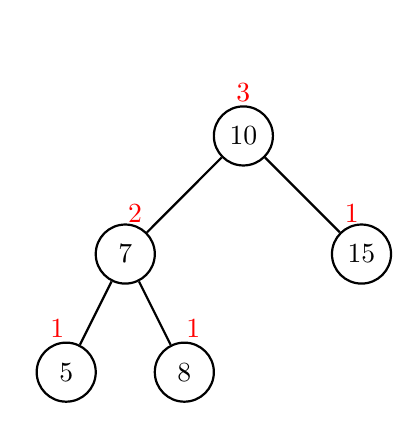
\begin{tikzpicture}[
  level distance=1.5 cm,
  level 1/.style={sibling distance=3cm},
  level 2/.style={sibling distance=1.5cm},
  minimum size=.75cm, thick]

  \node[circle,draw] (10){10}
	child {node[circle,draw]{7}
		child{node[circle,draw]{5}
			edge from parent node[near end, left, red]{1}}
		child{node[circle,draw]{8}
			edge from parent node[near end, right, red]{1}}
		edge from parent node[near end, left, red]{2}
	}
	child{node[circle,draw]{15}
		edge from parent node[near end, right, red]{1}
	};
   \node[draw=none, node distance=1cm](3)[above of=10]{};
   \draw[] (3) edge[draw=none, near start, red] node {3} (10);
\end{tikzpicture}

\end{center}
\end{columns}

\end{frame}


%------------------------------------------------

\begin{frame}
\frametitle{Left-Right and Right-Left}
\begin{columns}[c] 
\column{.35\textwidth}
\begin{itemize}
\only<1>{
\item The top is a Right-Left case
  \begin{itemize}
  \item A's right subtree is greater than A's left subtree
  \item C's left subtree is greater than C's right subtree
  \end{itemize}%
}
\only<2>{
\item The Left-Right case is the mirror opposite. 
\item Need two rotations.
}
\end{itemize}
\column{.5\textwidth}
\begin{center}

% right-left
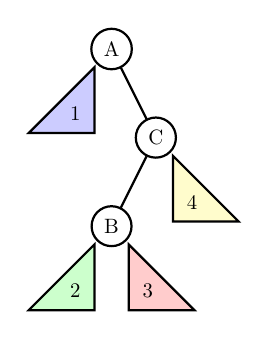
\begin{tikzpicture}[scale=.75, transform shape, level distance=1.5 cm, level 1/.style={sibling distance=1.5cm}, level 2/.style={sibling distance=1.5cm}, thick]
  \node[circle,draw] (A){A}
	child[fill=none] {edge from parent[draw=none]}
	child {node[circle,draw](C){C}
		child {node[circle,draw](B){B}}
		child[fill=none] {edge from parent[draw=none]}
		};
\node[draw, shape border uses incircle, isosceles triangle,isosceles triangle apex angle=90, shape border rotate=-45][below left of=A, anchor=north, node distance=0.87cm, fill=blue!20!]{1};
\node[draw, shape border uses incircle, isosceles triangle,isosceles triangle apex angle=90, shape border rotate=-45][below left of=B, anchor=north, node distance=0.87cm, fill=green!20!]{2};
\node[isosceles triangle, draw, shape border uses incircle, isosceles triangle,isosceles triangle apex angle=90, shape border rotate=225][below right of=B, anchor=north, node distance=0.87cm, fill=red!20!]{3};
\node[isosceles triangle, draw, shape border uses incircle, isosceles triangle,isosceles triangle apex angle=90, shape border rotate=225][below right of=C, anchor=north, node distance=0.87cm, fill=yellow!20!]{4};
\end{tikzpicture}


\vspace{.5cm}

% left-right
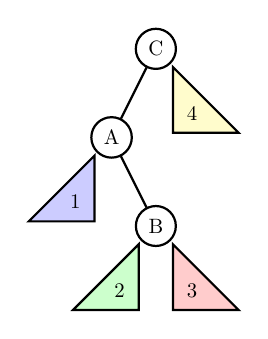
\begin{tikzpicture}[scale=.75, transform shape,
  level distance=1.5 cm,
  level 1/.style={sibling distance=1.5cm},
  level 2/.style={sibling distance=1.5cm},
  thick]

  \node[circle,draw] (C){C}
	child {node[circle,draw](A){A}
		child[fill=none] {edge from parent[draw=none]}		
		child {node[circle,draw](B){B}}
		}
	child[fill=none] {edge from parent[draw=none]};


    \node[draw, shape border uses incircle, isosceles triangle,isosceles triangle apex angle=90, shape border rotate=-45][below left of=A, anchor=north, node distance=0.87cm, fill=blue!20!]{1};
    \node[draw, shape border uses incircle, isosceles triangle,isosceles triangle apex angle=90, shape border rotate=-45][below left of=B, anchor=north, node distance=0.87cm, fill=green!20!]{2};
  \node[isosceles triangle, draw, shape border uses incircle, isosceles triangle,isosceles triangle apex angle=90, shape border rotate=225][below right of=B, anchor=north, node distance=0.87cm, fill=red!20!]{3};
  \node[isosceles triangle, draw, shape border uses incircle, isosceles triangle,isosceles triangle apex angle=90, shape border rotate=225][below right of=C, anchor=north, node distance=0.87cm, fill=yellow!20!]{4};
\end{tikzpicture}

\end{center}

\end{columns}
\end{frame}

%------------------------------------------------

\begin{frame}
\frametitle{Left-Right and Right-Left}
\begin{columns}[c] 
\column{.5\textwidth}
\begin{itemize}
\item Rotate right on C.
\end{itemize}

\column{.5\textwidth}
\begin{center}
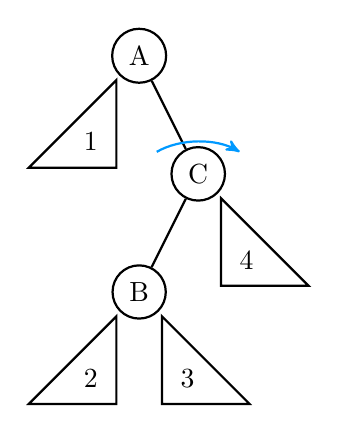
\begin{tikzpicture}[level distance=1.5 cm, node distance=.7cm, level 1/.style={sibling distance=1.5cm}, level 2/.style={sibling distance=1.5cm}, thick]
  \node[circle,draw] (A){A}
	child[fill=none] {edge from parent[draw=none]}
	child {node[circle,draw](C){C}
		child {node[circle,draw](B){B}}
		child[fill=none] {edge from parent[draw=none]}
		};
\node[draw, shape border uses incircle, isosceles triangle,isosceles triangle apex angle=90, shape border rotate=-45][below left of=A, anchor=north, node distance=0.87cm]{1};
\node[draw, shape border uses incircle, isosceles triangle,isosceles triangle apex angle=90, shape border rotate=-45][below left of=B, anchor=north, node distance=0.87cm]{2};
\node[isosceles triangle, draw, shape border uses incircle, isosceles triangle,isosceles triangle apex angle=90, shape border rotate=225][below right of=B, anchor=north, node distance=0.87cm]{3};
\node[isosceles triangle, draw, shape border uses incircle, isosceles triangle,isosceles triangle apex angle=90, shape border rotate=225][below right of=C, anchor=north, node distance=0.87cm]{4};  
\node[circle, draw=none] [left of=C](L){};
\node[circle, draw=none] [right of=C](R){};
\path[->, >=stealth', auto] (L.north) edge[bend left, shorten >=.2cm, shorten <=.2cm, blue!40!cyan ] (R.north);
\end{tikzpicture}
\end{center}

\end{columns}
\end{frame}



%-----------------------------------------------
\begin{frame}
\frametitle{Left-Right and Right-Left}
\begin{columns}[c] 
\column{.5\textwidth}
\begin{itemize}
\item The right subtree of B becomes the left subtree of C
\item C becomes the right child of B.
\item B becomes the right child of A.
\item Now a Right-Right case.
\item<2> Rotate left on A.
\end{itemize}
\column{.5\textwidth}
\begin{center}

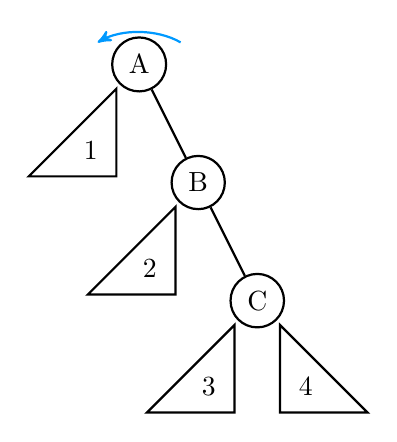
\begin{tikzpicture}[
  level distance=1.5 cm,
  node distance=.7cm,
  level 1/.style={sibling distance=1.5cm},
  level 2/.style={sibling distance=1.5cm},
  thick]

  \node[circle,draw] (A){A}
	child[fill=none] {edge from parent[draw=none]}
	child {node[circle,draw](B){B}
		child[fill=none] {edge from parent[draw=none]}		
		child {node[circle,draw](C){C}}
		};


  \node[draw, shape border uses incircle, isosceles triangle,isosceles triangle apex angle=90, shape border rotate=-45][below left of=A, anchor=north, node distance=0.87cm]{1};
  \node[draw, shape border uses incircle, isosceles triangle,isosceles triangle apex angle=90, shape border rotate=-45][below left of=B, anchor=north, node distance=0.87cm]{2};
  \node[draw, shape border uses incircle, isosceles triangle,isosceles triangle apex angle=90, shape border rotate=-45][below left of=C, anchor=north, node distance=0.87cm]{3};
  \node[isosceles triangle, draw, shape border uses incircle, isosceles triangle,isosceles triangle apex angle=90, shape border rotate=225][below right of=C, anchor=north, node distance=0.87cm]{4};
\only<2>{  
  \node[circle, draw=none] [left of=A](L){};
  \node[circle, draw=none] [right of=A](R){};
    \path[->, >=stealth', auto]
      (R.north) edge[bend right, shorten >=.2cm, shorten <=.2cm, blue!40!cyan ] (L.north);
      }
\end{tikzpicture}
\end{center}
\end{columns}
\end{frame}

%------------------------------------------------

\begin{frame}
\frametitle{Left-Right and Right-Left}
\begin{columns}[c] 
\column{.5\textwidth}
\begin{itemize}
\item The left subtree of B becomes the right subtree of A.
\item A becomes the left child of B.
\end{itemize}
\column{.5\textwidth}
\begin{center}
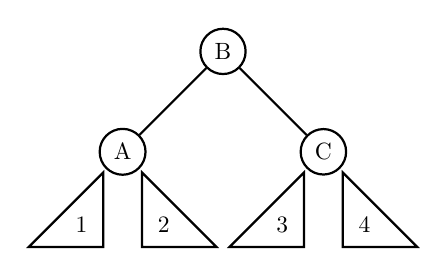
\begin{tikzpicture}[scale=.85, transform shape,
  level distance=1.5 cm,
  level 1/.style={sibling distance=3cm},
  level 2/.style={sibling distance=1.5cm},
  thick]

  \node[circle,draw] (B){B}
	child {node[circle,draw](A){A}}
	child {node[circle,draw](C){C}};

  \node[draw, shape border uses incircle, isosceles triangle,isosceles triangle apex angle=90, shape border rotate=-45](1)[below left of=A, anchor=north, node distance=0.87cm]{1};
    \node[isosceles triangle, draw, shape border uses incircle, isosceles triangle,isosceles triangle apex angle=90, shape border rotate=225](4)[below right of=A, anchor=north, node distance=0.87cm]{2};
  \node[draw, shape border uses incircle, isosceles triangle,isosceles triangle apex angle=90, shape border rotate=-45](2)[below left of=C, anchor=north, node distance=0.87cm]{3};
  \node[isosceles triangle, draw, shape border uses incircle, isosceles triangle,isosceles triangle apex angle=90, shape border rotate=225](4)[below right of=C, anchor=north, node distance=0.87cm]{4};
\end{tikzpicture}
\end{center}
\end{columns}
\end{frame}


%------------------------------------------------

\begin{frame}
\frametitle{Balance}
\begin{center}
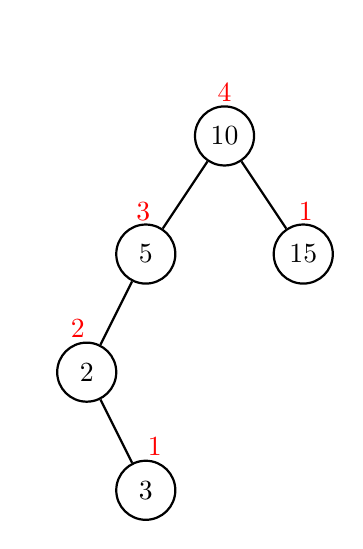
\begin{tikzpicture}[
  level distance=1.5 cm,
  level 1/.style={sibling distance=2cm},
  level 2/.style={sibling distance=1.5cm},
  level 3/.style={sibling distance=1.5cm},
  minimum size=.75cm, thick]

  \node[circle,draw](10) {10}
	child {node[circle,draw]{5}
		child{node[circle,draw]{2}
			child[fill=none] {edge from parent[draw=none]}
			child{node[circle,draw]{3}
				edge from parent node[near end, right, red]{1}
			}
			edge from parent node[near end, left, red]{2}	
		}	
		child[fill=none] {edge from parent[draw=none]}
		edge from parent node[near end, left, red]{3}
		}
	child{node[circle,draw]{15}
		edge from parent node[near end, right, red]{1}
	};
   \node[draw=none, node distance=1cm](4)[above of=10]{};
   \draw[] (4) edge[draw=none, near start, red] node {4} (10);
\end{tikzpicture}
\end{center}


\end{frame}
%------------------------------------------------
\begin{frame}
\frametitle{Balance}
\begin{columns}[c]
\column{.5\textwidth}
\begin{itemize}
\item 10's left subtree is out of balance
  \begin{itemize}
  \item 5's left subtree has a height of 2
  \item 5's right subtree has a height of 0.
  \end{itemize}
\item  Left-Right case 
  \begin{itemize}
  \item 2's right subtree is heavier than 2's left
  \end{itemize}
\item Rotate left on 2
\end{itemize}
\column{.5\textwidth}
\begin{center}

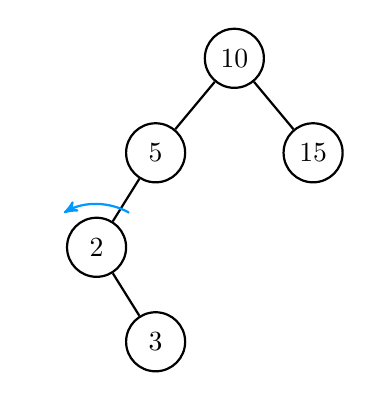
\begin{tikzpicture}[
  level distance=1.2 cm,
  node distance=.5cm,
  level 1/.style={sibling distance=2cm},
  level 2/.style={sibling distance=1.5cm},
  level 3/.style={sibling distance=1.5cm},
  minimum size=.75cm, thick]

  \node[circle,draw] {10}
	child {node[circle,draw]{5}
		child{node[circle,draw](2){2}
			child[fill=none] {edge from parent[draw=none]}
			child{node[circle,draw]{3}}	
		}	
		child[fill=none] {edge from parent[draw=none]}
		}
	child{node[circle,draw]{15}};
  \node[circle, draw=none] [left of=2](L){};
  \node[circle, draw=none] [right of=2](R){};
    \path[->, >=stealth', auto]
      (R.north) edge[bend right, shorten >=.1cm, shorten <=.1cm, blue!40!cyan ] (L.north);
\end{tikzpicture}
\end{center}
\end{columns}
\end{frame}
%---------------------------------------------------------------------------------
\begin{frame}
\frametitle{Balance}
\begin{columns}[c]

\column{.5\textwidth}
\begin{itemize}

\item 2 becomes the left child of 3
\item 3 becomes the left child of 5
\item Now a Left-Left case
\item Rotate right on 5

\end{itemize}
\column{.5\textwidth}
\begin{center}

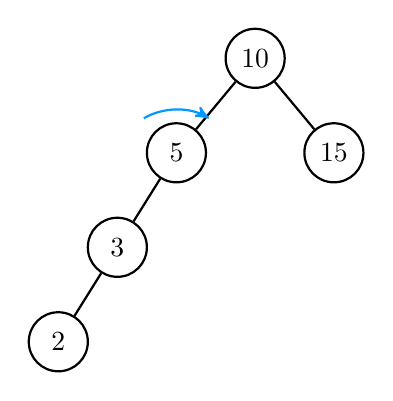
\begin{tikzpicture}[
  level distance=1.2 cm,
  node distance=.5cm,
  level 1/.style={sibling distance=2cm},
  level 2/.style={sibling distance=1.5cm},
  level 3/.style={sibling distance=1.5cm},
  minimum size=.75cm, thick]

  \node[circle,draw] {10}
	child {node[circle,draw](5){5}
		child{node[circle,draw]{3}
			child{node[circle,draw]{2}}
				child[fill=none] {edge from parent[draw=none]}
		}
		child[fill=none] {edge from parent[draw=none]}
	}
	child{node[circle,draw]{15}};
  \node[circle, draw=none] [left of=5](L){};
  \node[circle, draw=none] [right of=5](R){};
    \path[->, >=stealth', auto]
      (L.north) edge[bend left, shorten >=.1cm, shorten <=.1cm, blue!40!cyan ] (R.north);
\end{tikzpicture}

\end{center}
\end{columns}

\end{frame}
%------------------------------------------------
\begin{frame}
\frametitle{Balance}
\begin{columns}
\column{.5\textwidth}
\begin{itemize}
\item 5 becomes the right child of 3 
\item 3 becomes the left child of 10
\end{itemize}

\column{.5\textwidth}

\begin{center}

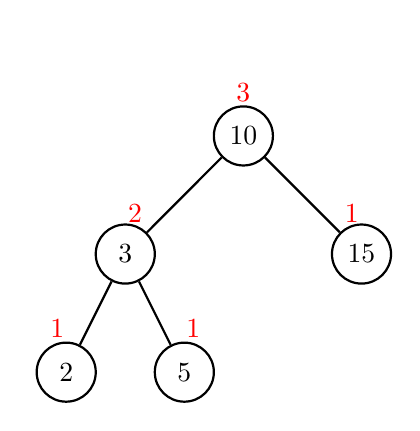
\begin{tikzpicture}[
  level distance=1.5 cm,
  level 1/.style={sibling distance=3cm},
  level 2/.style={sibling distance=1.5cm},
  minimum size=.75cm, thick]

  \node[circle,draw] (10){10}
	child {node[circle,draw]{3}
		child{node[circle,draw]{2}
			edge from parent node[near end, left, red]{1}}
		child{node[circle,draw]{5}
			edge from parent node[near end, right, red]{1}}
		edge from parent node[near end, left, red]{2}
	}
	child{node[circle,draw]{15}
		edge from parent node[near end, right, red]{1}
	};
   \node[draw=none, node distance=1cm](4)[above of=10]{};
   \draw[] (4) edge[draw=none, near start, red] node {3} (10);
\end{tikzpicture}

\end{center}
\end{columns}
\end{frame}

%------------------------------------------------
\begin{frame}
\frametitle{AVL}
\begin{itemize}
\item  Balance everytime you insert or remove a node to keep the tree balanced at every step.
\item This will always give one of the cases shown.
\end{itemize}
\end{frame}

%------------------------------------------------
\begin{frame}
\frametitle{Inserting into AVL trees}
\begin{itemize}
\item Start at the root and trace through until you reach a leaf node.
\item Create a node with the new information and make it either the left or right child of the leaf node.
\item Rebalance at each level.
\end{itemize}
\end{frame}

%------------------------------------------------

\begin{frame}
\frametitle{Insert 33}

\begin{center}

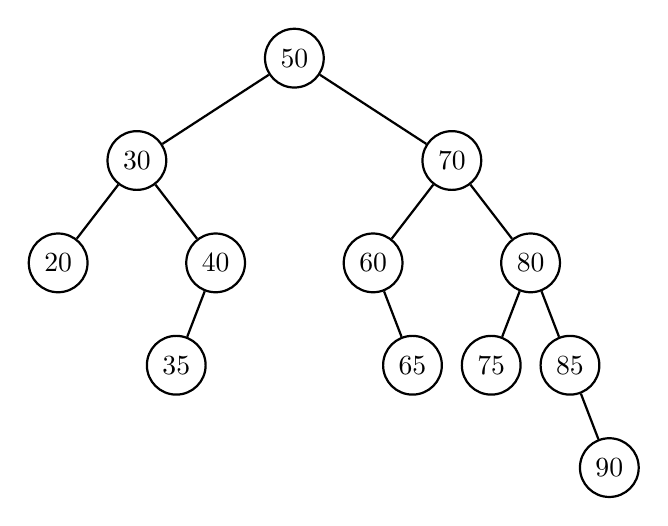
\begin{tikzpicture}[
  level distance=1.3 cm,
  level 1/.style={sibling distance=4cm}, % Adjust the level distance to compensate for additional nodes
  level 2/.style={sibling distance=2cm},
  level 3/.style={sibling distance=1cm},
   thick]

  \node[circle,draw] {50}
	child {node[circle,draw]{30}
		child{node[circle,draw]{20}}
		child{node[circle,draw]{40}
			child{node[circle,draw]{35}}
			child[fill=none] {edge from parent[draw=none]} 
		}
	}
	child{node[circle,draw]{70}
		child{node[circle,draw]{60}
			child[fill=none] {edge from parent[draw=none]} 
			child{node[circle,draw]{65}}
		}
		child{node[circle,draw]{80}
			child{node[circle,draw]{75}}
			child{node[circle,draw]{85}
				child[fill=none] {edge from parent[draw=none]} 
				child{node[circle,draw]{90}}	
			}
		}
	};
\end{tikzpicture}

\end{center}

\end{frame}
%------------------------------------------------

\begin{frame}
\frametitle{Insert 33}
\begin{columns}[c]
\column{.3\textwidth}
\begin{itemize}

\item 33 becomes the left child of 35
\item Left-Left case.
\item<2->  Rotate right on 40.

\end{itemize}

\column{.7\textwidth}
\begin{center}

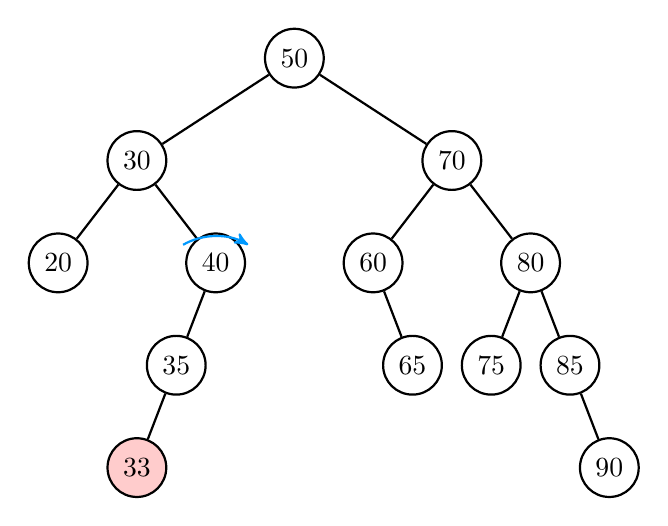
\begin{tikzpicture}[
  node distance = .5cm,
  level distance=1.3 cm,
  level 1/.style={sibling distance=4cm}, % Adjust the level distance to compensate for additional nodes
  level 2/.style={sibling distance=2cm},
  level 3/.style={sibling distance=1cm},
   thick]

  \node[circle,draw] {50}
	child {node[circle,draw]{30}
		child{node[circle,draw]{20}}
		child{node[circle,draw](40){40}
			child{node[circle,draw]{35}
				child{node[circle,draw,fill=red!20!]{33}}
				child[fill=none]{edge from parent[draw=none]}
			}
			child[fill=none] {edge from parent[draw=none]} 
		}
	}
	child{node[circle,draw]{70}
		child{node[circle,draw]{60}
			child[fill=none] {edge from parent[draw=none]} 
			child{node[circle,draw]{65}}
		}
		child{node[circle,draw]{80}
			child{node[circle,draw]{75}}
			child{node[circle,draw]{85}
				child[fill=none] {edge from parent[draw=none]} 
				child{node[circle,draw]{90}}	
			}
		}
	};
\only<2->{
  \node[circle, draw=none] [left of=40](L){};
  \node[circle, draw=none] [right of=40](R){};
    \path[->, >=stealth', auto]
      (L.north) edge[bend left, shorten >=.1cm, shorten <=.1cm, blue!40!cyan ] (R.north); %FIX ME!!!!!!!!!!!!!!!!!!!
 }
\end{tikzpicture}

\end{center}
\end{columns}

\end{frame}
%------------------------------------------------


\begin{frame}
\frametitle{Insert 33}

\begin{columns}[c]
\column{.3\textwidth}
\begin{itemize}

\item 35 becomes the parent with 40 as a right child and 33 as a left child.
\end{itemize}
\column{.7\textwidth}
\begin{center}

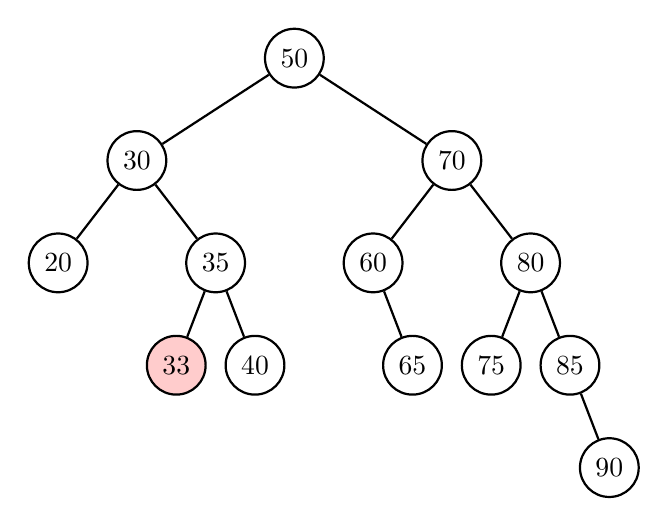
\begin{tikzpicture}[
  level distance=1.3 cm,
  level 1/.style={sibling distance=4cm}, % Adjust the level distance to compensate for additional nodes
  level 2/.style={sibling distance=2cm},
  level 3/.style={sibling distance=1cm},
   thick]

  \node[circle,draw] {50}
	child {node[circle,draw]{30}
		child{node[circle,draw]{20}}
		child{node[circle,draw]{35}
			child{node[circle,draw,fill=red!20!]{33}}
			child{node[circle,draw]{40}}
		}
	}
	child{node[circle,draw]{70}
		child{node[circle,draw]{60}
			child[fill=none] {edge from parent[draw=none]} 
			child{node[circle,draw]{65}}
		}
		child{node[circle,draw]{80}
			child{node[circle,draw]{75}}
			child{node[circle,draw]{85}
				child[fill=none] {edge from parent[draw=none]} 
				child{node[circle,draw]{90}}	
			}
		}
	};
\end{tikzpicture}

\end{center}
\end{columns}
\end{frame}

%------------------------------------------------

\begin{frame}
\frametitle{Deleting from AVL Trees}
\begin{itemize}
\item Start at the root and trace through until you find the node to delete.
\item If you reach a leaf node without finding it, the node is not in the tree.
\item Tthree cases: zero, one, or two children.
\end{itemize}
\end{frame}

%------------------------------------------------
\begin{frame}
\frametitle{Deleting a Leaf Node}
\begin{columns}[c]
\column{.3\textwidth}
\begin{itemize}
\item Simply delete it and rebalance.
\item Delete 8.
\end{itemize}
\column{.7\textwidth}
\begin{center}

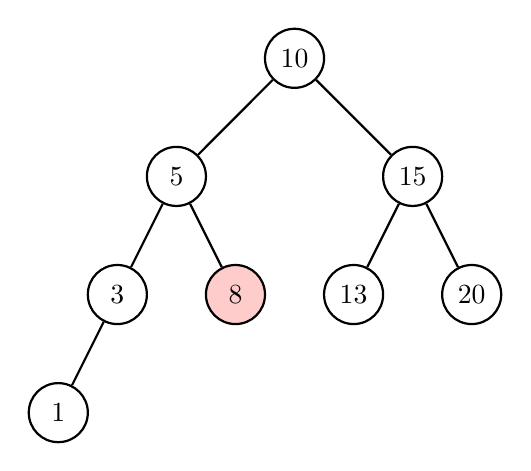
\begin{tikzpicture}[
  level distance=1.5 cm,
  level 1/.style={sibling distance=3cm},
  level 2/.style={sibling distance=1.5cm},
  level 3/.style={sibling distance=1.5cm},
  minimum size=.75cm, thick]

  \node[circle,draw] {10}
	child {node[circle,draw]{5}
		child{node[circle,draw]{3}
			child{node[circle,draw]{1}}
			child[fill=none]{edge from parent[draw=none]}
		}
		child{node[circle,draw,fill=red!20!]{8}
		}
	}
	child{node[circle,draw]{15}
		child{node[circle,draw]{13}
		}
		child{node[circle,draw]{20}
		}
	};
\end{tikzpicture}
\end{center}
\end{columns}
\end{frame}
%------------------------------------------------
\begin{frame}
\frametitle{Deleting a Leaf Node}
\begin{columns}[c]
\column{.3\textwidth}
\begin{itemize}
\item 5 is out of balance
\item Left-Left case
\item Rotate right on 5
\end{itemize}
\column{.7\textwidth}

\begin{center}

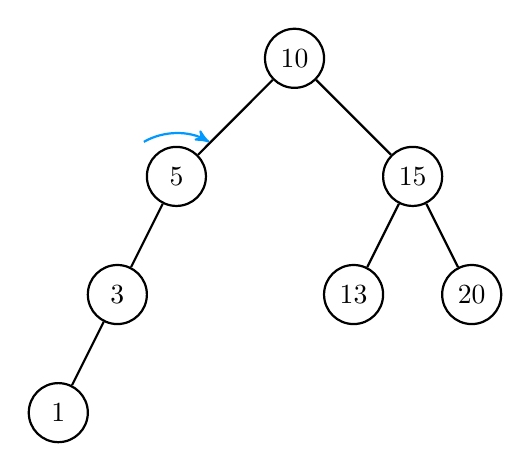
\begin{tikzpicture}[
  level distance=1.5 cm,
  node distance=.5cm,
  level 1/.style={sibling distance=3cm},
  level 2/.style={sibling distance=1.5cm},
  level 3/.style={sibling distance=1.5cm},
  minimum size=.75cm, thick]

  \node[circle,draw] {10}
	child {node[circle,draw](5){5}
		child{node[circle,draw]{3}
			child{node[circle,draw]{1}}
			child[fill=none]{edge from parent[draw=none]}
		}
		child[fill=none]{edge from parent[draw=none]
		}
	}
	child{node[circle,draw]{15}
		child{node[circle,draw]{13}
		}
		child{node[circle,draw]{20}
		}
	};
  \node[circle, draw=none] [left of=5](L){};
  \node[circle, draw=none] [right of=5](R){};
    \path[->, >=stealth', auto]
      (L.north) edge[bend left, shorten >=.1cm, shorten <=.1cm, blue!40!cyan ] (R.north);
\end{tikzpicture}

\end{center}

\end{columns}
\end{frame}
%------------------------------------------------
\begin{frame}
\frametitle{Deleting a Leaf Node}

\begin{center}

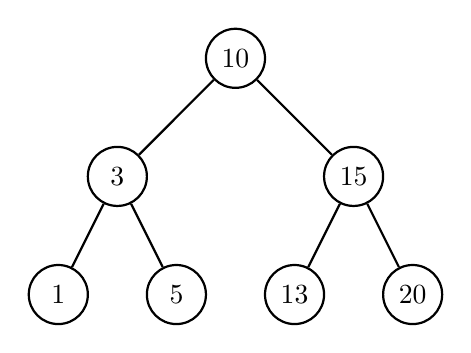
\begin{tikzpicture}[
  level distance=1.5 cm,
  level 1/.style={sibling distance=3cm},
  level 2/.style={sibling distance=1.5cm},
  minimum size=.75cm, thick]

  \node[circle,draw] {10}
	child {node[circle,draw]{3}
		child{node[circle,draw]{1}
		}
		child{node[circle,draw]{5}
		}
	}
	child{node[circle,draw]{15}
		child{node[circle,draw]{13}
		}
		child{node[circle,draw]{20}
		}
	};
\end{tikzpicture}

\end{center}


\end{frame}
%------------------------------------------------
\begin{frame}
\frametitle{Deleting a Node with One Child}
\begin{itemize}
\item Simply deleting will lose the child
\item Replace the node with its child
\item Rebalance
\end{itemize}

\end{frame}
%------------------------------------------------
\begin{frame}
\frametitle{Deleting a Node with One Child}
Delete 19
\begin{center}
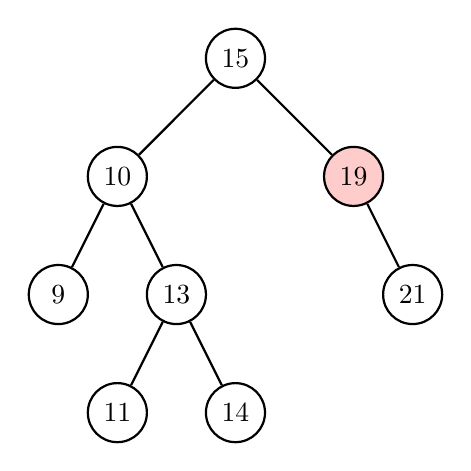
\begin{tikzpicture}[
  level distance=1.5 cm,
  level 1/.style={sibling distance=3cm},
  level 2/.style={sibling distance=1.5cm},
  level 3/.style={sibling distance=1.5cm},
  minimum size=.75cm, thick]

  \node[circle,draw] {15}
	child {node[circle,draw]{10}
		child{node[circle,draw]{9}
		}
		child{node[circle,draw]{13}
			child{node[circle, draw]{11}}
			child{node[circle, draw]{14}}
		}
	}
	child{node[circle,draw, fill=red!20!]{19}
		child[fill=none] {edge from parent[draw=none]}
		child{node[circle,draw]{21}}
	};
\end{tikzpicture}
\end{center}
\end{frame}
%-----------------------------------------------
\begin{frame}
\frametitle{Deleting a Node with One Child}
\begin{columns}[c]
\column{.5\textwidth}
\begin{itemize}
\item Delete 19
\item Move 21 to be the right child of 15
\item15 out of balance
  \begin{itemize}
  \item difference of 2 between 15's left and right subtrees
  \end{itemize}
\end{itemize}

\column{.5\textwidth}
\begin{center}

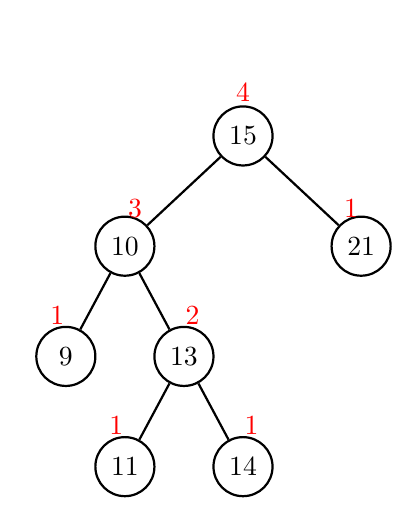
\begin{tikzpicture}[
  level distance=1.4 cm,
  node distance=.5cm,
  level 1/.style={sibling distance=3cm},
  level 2/.style={sibling distance=1.5cm},
  level 3/.style={sibling distance=1.5cm},
  minimum size=.75cm, thick]

  \node[circle,draw](15){15}
	child {node[circle,draw](10){10}
		child{node[circle,draw]{9}
			edge from parent node[near end, left, red]{1}
		}
		child{node[circle,draw]{13}
			child{node[circle, draw] {11}
				edge from parent node[near end, left, red]{1}}
			child{node[circle, draw]{14}
				edge from parent node[near end, right, red]{1}}
			edge from parent node[near end, right, red]{2}
		}
	edge from parent node[near end, left, red]{3}
	}
	child{node[circle,draw]{21}
		edge from parent node[near end, right, red]{1}
	};
   \node[draw=none, node distance=1cm](4)[above of=15]{};
   \draw[] (4) edge[draw=none, near start, red] node {4} (15);
\end{tikzpicture}

\end{center}
\end{columns}
\end{frame}
%-----------------------------------------------
\begin{frame}
\frametitle{Deleting a Node with One Child}
\begin{columns}[c]
\column{.5\textwidth}
\begin{itemize}
\item Left-Right case 
  \begin{itemize}
  \item15's left subtree is heavier
  \item10's right subtree is heavier
  \end{itemize}
\item Rotate left on 10
\end{itemize}

\column{.5\textwidth}
\begin{center}

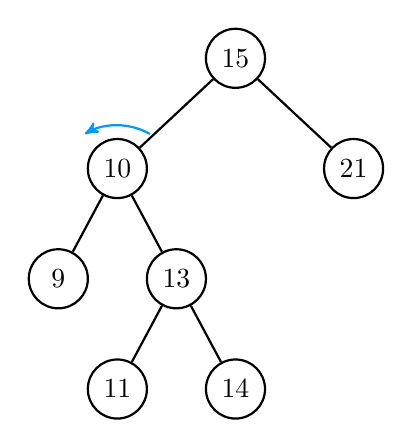
\begin{tikzpicture}[
  level distance=1.4 cm,
  node distance=.5cm,
  level 1/.style={sibling distance=3cm},
  level 2/.style={sibling distance=1.5cm},
  level 3/.style={sibling distance=1.5cm},
  minimum size=.75cm, thick]

  \node[circle,draw](15){15}
	child {node[circle,draw](10){10}
		child{node[circle,draw]{9}
		}
		child{node[circle,draw]{13}
			child{node[circle, draw] {11}}
			child{node[circle, draw]{14}}
		}
	}
	child{node[circle,draw]{21}
	};
  \node[circle, draw=none] [left of=10](L){};
  \node[circle, draw=none] [right of=10](R){};
    \path[->, >=stealth', auto]
      (R.north) edge[bend right, shorten >=.1cm, shorten <=.1cm, blue!40!cyan ] (L.north);
\end{tikzpicture}

\end{center}
\end{columns}
\end{frame}
%------------------------------------------------------------
\begin{frame}
\frametitle{Deleting a Node with One Child}
\begin{columns}[c]
\column{.5\textwidth}
\begin{itemize}
\item<1-> Left-Left case
\item<2-> Rotate right on 15
\end{itemize}

\column{.5\textwidth}
\begin{center}

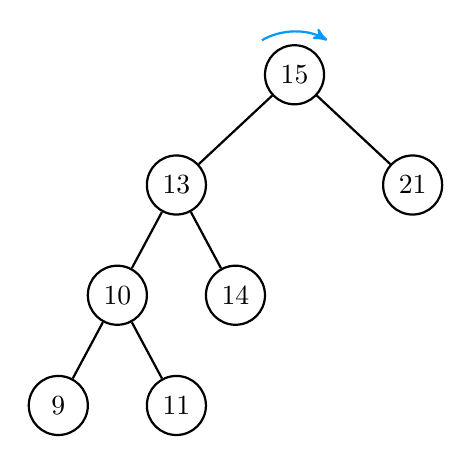
\begin{tikzpicture}[
  level distance=1.4 cm,
  node distance=.5cm,
  level 1/.style={sibling distance=3cm},
  level 2/.style={sibling distance=1.5cm},
  level 3/.style={sibling distance=1.5cm},
  minimum size=.75cm, thick]

  \node[circle,draw](15) {15}
	child {node[circle,draw]{13}
		child{node[circle,draw]{10}
			child{node[circle,draw]{9}}
			child{node[circle,draw]{11}}
		}
		child{node[circle,draw]{14}
		}
	}
	child{node[circle,draw]{21}
	};
\only<2->{
  \node[circle, draw=none] [left of=15](L){};
  \node[circle, draw=none] [right of=15](R){};
    \path[->, >=stealth', auto]
      (L.north) edge[bend left, shorten >=.1cm, shorten <=.1cm, blue!40!cyan ] (R.north);
      }

\end{tikzpicture}

\end{center}
\end{columns}
\end{frame}
%------------------------------------------------
\begin{frame}
\frametitle{Deleting a Node with One Child}

\begin{center}

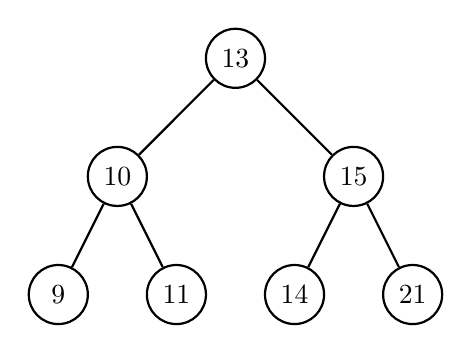
\begin{tikzpicture}[
  level distance=1.5 cm,
  level 1/.style={sibling distance=3cm},
  level 2/.style={sibling distance=1.5cm},
  minimum size=.75cm, thick]

  \node[circle,draw] {13}
	child {node[circle,draw]{10}
		child{node[circle,draw]{9}}
		child{node[circle,draw]{11}}
	}
	child{node[circle,draw]{15}
		child{node[circle,draw]{14}}
		child{node[circle,draw]{21}}
	};
\end{tikzpicture}

\end{center}

\end{frame}

%------------------------------------------------

\begin{frame}
\frametitle{Deleting a Node with Two Children}
\begin{itemize}
\item Replace it with the in-order successor or the in-order predecessor, using one of the simpler cases.
\item Rebalance.
\item The in-order successor is the left-most child of the right subtree
\item The in-order predecessor is the right-most child of the left subtree. 
\item Pick one and use it every time. Here, we use the in-order sucessor.
\end{itemize}
\end{frame}


%------------------------------------------------
\begin{frame}
\frametitle{Deleting a Node with Two Children}

Delete 14

\begin{center}
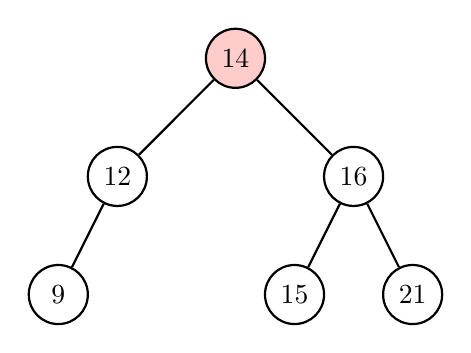
\begin{tikzpicture}[
  level distance=1.5 cm,
  level 1/.style={sibling distance=3cm},
  level 2/.style={sibling distance=1.5cm},
  minimum size=.75cm, thick]

  \node[circle,draw,fill=red!20!] {14}
	child {node[circle,draw]{12}
		child{node[circle,draw]{9}}
		child[fill=none] {edge from parent[draw=none]} 
	}
	child{node[circle,draw]{16}
		child{node[circle,draw]{15}}
		child{node[circle,draw]{21}}
	};
\end{tikzpicture}
\end{center}
\end{frame}
%------------------------------------------------
\begin{frame}
\frametitle{Deleting a Node with Two Children}
\begin{columns}[c]
\column{.5\textwidth}
\begin{itemize}
\item Find the in-order successor by tracing through the right subtree.
\item Choose the left until there are no more left children.
\item The in-order sucessor is 15.
\end{itemize}
\column{.5\textwidth}
\begin{center}

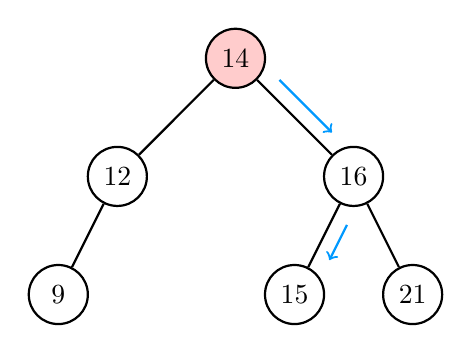
\begin{tikzpicture}[
  level distance=1.5 cm,
  level 1/.style={sibling distance=3cm},
  level 2/.style={sibling distance=1.5cm},
  minimum size=.75cm, thick]
  
   \pgfdeclaredecoration{sl}{initial}{
  \state{initial}[width=\pgfdecoratedpathlength-1sp]{
     \pgfmoveto{\pgfpointorigin}
  }
  \state{final}{
     \pgflineto{\pgfpointorigin}
    }
}

\tikzset{parallel arrow/.style={->, 
     shorten >=2mm, shorten <=2mm, 
     decoration={sl,raise=.2cm}, blue!40!cyan, decorate}}

  \node[circle,draw,fill=red!20!](14){14}
	child {node[circle,draw]{12}
		child{node[circle,draw]{9}}
		child[fill=none] {edge from parent[draw=none]} 
	}
	child{node[circle,draw](16){16}
		child{node[circle,draw](15){15}}
		child{node[circle,draw]{21}}
	};

  \draw[] (14) edge[parallel arrow] node {} (16);
  \draw[] (16) edge[parallel arrow] node {}  (15);
\end{tikzpicture}

\end{center}
\end{columns}
\end{frame}
%------------------------------------------------
\begin{frame}
\frametitle{Deleting a Node with Two Children}
\begin{columns}[c]
\column{.5\textwidth}
\begin{itemize}
\item Switch the in-order sucessor with 14 and delete the leaf node.
\item Start at the leaf node and rebalance all the way up.
\end{itemize}
\column{.5\textwidth}
\begin{center}

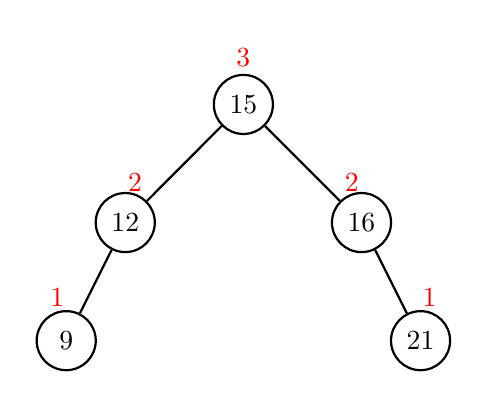
\begin{tikzpicture}[
  level distance=1.5 cm,
  level 1/.style={sibling distance=3cm},
  level 2/.style={sibling distance=1.5cm},
  minimum size=.75cm, thick]

  \node[circle,draw] (15){15}
	child {node[circle,draw]{12}
		child{node[circle,draw]{9}
			edge from parent node[near end, left, red]{1}}
		child[fill=none] {edge from parent[draw=none]} 
		edge from parent node[near end, left, red]{2}
	}
	child{node[circle,draw]{16}
		child[fill=none] {edge from parent[draw=none]} 
		child{node[circle,draw]{21}
			edge from parent node[near end, right, red]{1}}
		edge from parent node[near end, right, red]{2}
	};
  \node[draw=none, node distance=.6cm, red](3)[above of=15]{3};
\end{tikzpicture}

\end{center}
\end{columns}

\end{frame}

%------------------------------------------------
%B TREES %%%%%%%%%%%%%%%%%%%%%%%%%%%%%%%%%%%%%%%%%%%%%%%%%%%%
\begin{frame}
\frametitle{B trees}
\begin{itemize}
\item B-Trees are a very efficient form of balanced tree.
\item B-Trees relax the requirement of only two children per node.
\item Balance is achieved when all leaf nodes are at the same depth.
\item Split and join nodes to maintain balance.
\item Used in a variety of settings including databases and filesystems.
\end{itemize}
\end{frame}

%------------------------------------------------

\begin{frame}
\frametitle{B-Tree Example}
\begin{center}

\begin{tikzpicture}[
  level distance=1.5 cm,
  level 1/.style={sibling distance=3cm},
  thick]

  \node[bnode]{\nodepart{one}20 \nodepart{two}48 \nodepart{three}~ \nodepart{four}~}
	child[parent anchor=south west] 
	{node[bnode](lchild) {\nodepart{one}10 \nodepart{two}14 \nodepart{three}~ \nodepart{four}~ }}
	child[parent anchor = one split south]
	{node[bnode]{\nodepart{one}24 \nodepart{two}34\nodepart{three}~ \nodepart{four}~}}
	child[parent anchor = two split south, child anchor = north west]
	{node[bnode]{\nodepart{one}50 \nodepart{two}75\nodepart{three}99 \nodepart{four}~}
	};

\end{tikzpicture}

\end{center}
\end{frame}

%------------------------------------------------
\begin{frame}
\frametitle{Rules of B Trees}
\begin{itemize}
\item order $n$ means every node has at most $n$ children.
\item Every node, except for the root, has at least $n/2$ keys.
\item The root has at least 2 children (unless it is a leaf).
\item \label{enum:infoleaf} All leaves appear on the same level.
\item A nonleaf node with $n$ children contains $n-1$ keys.
\end{itemize}
\end{frame}

%------------------------------------------------
\begin{frame}
\frametitle{B Tree Attributes}
\begin{itemize}
\item The number of keys that a single B-Tree can hold grows exponentially with each new level of the tree.
\item A B-Tree of depth, $d$, and order $n$ can store a maximum of $n^{d} - 1$ keys.
\item A B-Tree of order 100 and depth 3 can store 999999 keys.
\item Adding a new level increases the total capacity one hundred fold, or 99999999 keys!
\end{itemize}
\end{frame}
%----------------------------------------------------
\begin{frame}
\frametitle{B Tree Attributes}
\begin{itemize}
\item  B-Trees are built from the bottom up (starting with a single leaf node). 
\item As more leaves are added, the root changes from a leaf node to an index node. 
\item In a B+Tree, the actual data of the tree is stored only in the bottom most nodes, or leaf nodes. All other nodes in the tree are index nodes.
\end{itemize}
\end{frame}
%-------------------------------------------------
\begin{frame}
\frametitle{Classwork}
\begin{itemize}
\item What is the maximum number of keys that a B-Tree of order $n$ and depth $d$ can hold?
\item<2-> $n^{d}-1$.
\item What is the maximum number of keys an AVL tree of depth $d$ can store?
\item <3-> $2^{d} -1$.
\end{itemize}
\end{frame}

%------------------------------------------------
\begin{frame}
\frametitle{Insertion into a not full leaf node}
\begin{itemize}
\item Trace through the tree starting at the root until you find the leaf node that should contain the new key.
\item If the leaf node is not full, insert the key without rearranging the tree.
\item If the leaf node is full, split it into two new leaf nodes.
\end{itemize}
\end{frame}
%------------------------------------------------

\begin{frame}
\frametitle{Insert 12}
\begin{center}
\begin{tikzpicture}[
  level distance=1.5 cm,
  level 1/.style={sibling distance=3cm},
  thick]

  \node[bnode]{\nodepart{one}17 \nodepart{two}~ \nodepart{three}~ \nodepart{four}~}
	child[parent anchor=south west] 
	{node[bnode](lchild) {\nodepart{one}2 \nodepart{two}15 \nodepart{three}~ \nodepart{four}~ }}
	child[parent anchor = one split south, child anchor = north west]
	{node[bnode]{\nodepart{one}21 \nodepart{two}33\nodepart{three}~ \nodepart{four}~}
	};
\end{tikzpicture}


\end{center}

\end{frame}
%------------------------------------------------
\begin{frame}
\frametitle{Insert 12}
\begin{columns}[c]
\column{.5\textwidth}
\begin{itemize}
\item Starting at the root, check 12 against 17
\item 12 is less than 17
\item go to the left child
\item The leaf node is not full, add 12.
\end{itemize}
\column{.5\textwidth}
\begin{center}


\begin{tikzpicture}[
  level distance=1.5 cm,
  level 1/.style={sibling distance=3cm},
  thick]

  \node[bnode]{\nodepart{one}17 \nodepart{two}~ \nodepart{three}~ \nodepart{four}~}
	child[parent anchor=south west] 
	{node[bnode](lchild) {\nodepart{one}2 \nodepart{two}\textbf{12} \nodepart{three}15 \nodepart{four}~ }}
	child[parent anchor = one split south, child anchor = north west]
	{node[bnode]{\nodepart{one}21 \nodepart{two}33\nodepart{three}~ \nodepart{four}~}
	};
\end{tikzpicture}

\end{center}
\end{columns}
\end{frame}
%------------------------------------------------

\begin{frame}
\frametitle{Insertion into a full leaf node}
\begin{itemize}
\item Insert the new key.
\item Find the median key
\item Promote meadian to the parent node.
\item All keys greater than the median key belong to the new right leaf node and all keys smaller than the median key belong to the new left leaf node.
\item If the parent node is full, split it by finding the median and promoting it.
\item Continue this process until you reach the root of the tree.
\end{itemize}
\end{frame}

%------------------------------------------------

\begin{frame}
\frametitle{Insert 5}
\begin{center}

\begin{tikzpicture}[
  level distance=1.5 cm,
  level 1/.style={sibling distance=3cm},
  thick]

  \node[bnode]{\nodepart{one}17 \nodepart{two}~ \nodepart{three}~ \nodepart{four}~}
	child[parent anchor=south west] 
	{node[bnode](lchild) {\nodepart{one}2 \nodepart{two}12 \nodepart{three}15 \nodepart{four}16 }}
	child[parent anchor = one split south, child anchor = north west]
	{node[bnode]{\nodepart{one}21 \nodepart{two}33\nodepart{three}~ \nodepart{four}~}
	};
\end{tikzpicture}

\end{center}

\end{frame}
%------------------------------------------------

\begin{frame}
\frametitle{Insert 5}
\begin{columns}[c]
\column{.4\textwidth}
\begin{itemize}
\item Insert 5
\item Find the median, 12.
\end{itemize}

\column{.6\textwidth}
\begin{center}

\begin{tikzpicture}[scale=.85, transform shape,
  level distance=1.5 cm,
  level 1/.style={sibling distance=4cm},
  thick]

  \node[bnode]{\nodepart{one}17 \nodepart{two}~ \nodepart{three}~ \nodepart{four}~}
	child[parent anchor=south west] 
	{node[bnode, rectangle split parts=5](lchild) {\nodepart{one}2 \nodepart{two}5 \nodepart{three}12 \nodepart{four}15 \nodepart{five}16}}
	child[parent anchor = one split south, child anchor = north west]
	{node[bnode]{\nodepart{one}21 \nodepart{two}33\nodepart{three}~ \nodepart{four}~}
	};
\node[draw=none](arrow)[below of = lchild]{};
\draw[->, thick, blue!40!cyan](arrow) -- (lchild);
\end{tikzpicture}


\end{center}

\end{columns}

\end{frame}


%----------------------------------------------------------------
\begin{frame}
\frametitle{Insert 5}
\begin{columns}[c]
\column{.35\textwidth}
\begin{itemize}
\item Promote median to parent. 
\item Split leaf node.
\end{itemize}

\column{.65\textwidth}
\begin{center}


\begin{tikzpicture}[scale=.85, transform shape,
  level distance=1.5 cm,
  level 1/.style={sibling distance=3cm},
  thick]

  \node[bnode]{\nodepart{one}12 \nodepart{two}17 \nodepart{three}~ \nodepart{four}~}
	child[parent anchor=south west] 
	{node[bnode](lchild) {\nodepart{one}2 \nodepart{two}5 \nodepart{three}~ \nodepart{four}~ }}
	child[parent anchor = one split south]
	{node[bnode]{\nodepart{one}15 \nodepart{two}16\nodepart{three}~ \nodepart{four}~}}
	child[parent anchor = two split south, child anchor = north west]
	{node[bnode]{\nodepart{one}21 \nodepart{two}33\nodepart{three}~ \nodepart{four}~}
	};

\end{tikzpicture}


\end{center}

\end{columns}

\end{frame}

%------------------------------------------------

\begin{frame}
\frametitle{Insert 18}
\begin{center}
\begin{tikzpicture}[scale=.8, transform shape,
  level distance=1.5 cm,
  level 1/.style={sibling distance=3cm},
  thick]
  \node[bnode] {\nodepart{one}3 \nodepart{two}6 \nodepart{three}12 \nodepart{four}19}
	child[parent anchor = south west]
	{node[bnode]{\nodepart{one}0 \nodepart{two}2 \nodepart{three}~ \nodepart{four}~}}
	child[parent anchor = one split south]
	{node[bnode]{\nodepart{one}4 \nodepart{two}5 \nodepart{three}~ \nodepart{four}~}}
	child[parent anchor = two split south]
	{node[bnode]{\nodepart{one}7 \nodepart{two}10 \nodepart{three}11 \nodepart{four}~}}
	child[parent anchor = three split south]
	{node[bnode] (node) {\nodepart{one}13 \nodepart{two}15 \nodepart{three}16 \nodepart{four}17}}
	child[parent anchor = south east]
	{node[bnode]{\nodepart{one}22 \nodepart{two}23 \nodepart{three}24 \nodepart{four}25}
	};
\end{tikzpicture}
\end{center}


\end{frame}


%------------------------------------------------

\begin{frame}
\frametitle{Insert 18}

\begin{center}

\begin{tikzpicture}[scale=.6, transform shape,
  level distance=1.5 cm,
  level 1/.style={sibling distance=4cm},
  thick]
  \node[bnode] {\nodepart{one}3 \nodepart{two}6 \nodepart{three}12 \nodepart{four}19}
	child[parent anchor = south west]
	{node[bnode]{\nodepart{one}0 \nodepart{two}2 \nodepart{three}~ \nodepart{four}~}}
	child[parent anchor = one split south]
	{node[bnode]{\nodepart{one}4 \nodepart{two}5 \nodepart{three}~ \nodepart{four}~}}
	child[parent anchor = two split south]
	{node[bnode]{\nodepart{one}7 \nodepart{two}10 \nodepart{three}11 \nodepart{four}~}}
	child[parent anchor = three split south]
	{node[bnode, rectangle split parts=5] (node) {\nodepart{one}13 \nodepart{two}15 \nodepart{three}16 \nodepart{four}17 \nodepart{five}\textbf{18}}}
	child[parent anchor = south east]
	{node[bnode]{\nodepart{one}22 \nodepart{two}23 \nodepart{three}24 \nodepart{four}25}
	};
  \node[draw=none] (arrow) [below of=node]{}; 
  \draw[->, thick, blue!40!cyan] (arrow) edge (node);
\end{tikzpicture}
\end{center}

Insert 18, find the median and split.


\end{frame}
%-------------------------------------------------
\begin{frame}
\frametitle{Insert 18}

\begin{center}

\begin{tikzpicture}[scale=.65, transform shape,
  level distance=1.5 cm,
  level 1/.style={sibling distance=3cm}, 
  thick]

  \node(root)[bnode, rectangle split parts=5] {\nodepart{one}3 \nodepart{two}6 \nodepart{three}12 \nodepart{four}16 \nodepart{five}19}
	child[parent anchor = south west]
	{node[bnode]{\nodepart{one}0 \nodepart{two}2 \nodepart{three}~ \nodepart{four}~}}
	child[parent anchor = one split south]
	{node[bnode]{\nodepart{one}4 \nodepart{two}5 \nodepart{three}~ \nodepart{four}~}}
	child[parent anchor = two split south]
	{node[bnode]{\nodepart{one}7 \nodepart{two}10 \nodepart{three}11 \nodepart{four}~}}
	child[parent anchor = three split south]
	{node[bnode] (node) {\nodepart{one}13 \nodepart{two}15 \nodepart{three}~ \nodepart{four}~ }}
	child[parent anchor = four split south]
	{node[bnode]{\nodepart{one}17 \nodepart{two}18 \nodepart{three}~ \nodepart{four}~}}
	child[parent anchor = south east]
	{node[bnode]{\nodepart{one}22 \nodepart{two}23 \nodepart{three}24 \nodepart{four}25}
	};

   \node[draw=none](arrow)[above of = root]{};
   \draw[->, thick,blue!40!cyan](arrow) edge (root);
\end{tikzpicture}
\end{center}


Find the median and split the root.



\end{frame}


%-------------------------------------------------
\begin{frame}
\frametitle{Insert 18}

\begin{center}

\begin{tikzpicture}[scale=.65, transform shape,
  level distance=1.5 cm,
  level 1/.style={sibling distance=9cm}, 
  level 2/.style={sibling distance=3cm},
  thick]

  \node(root)[bnode]{\nodepart{one}12\nodepart{two}~\nodepart{three}~\nodepart{four}~}
	  child[parent anchor = south west]
	  {node[bnode] {\nodepart{one}3 \nodepart{two}6 \nodepart{three}~ \nodepart{four}~ }
		child[parent anchor = south west]
		{node[bnode]{\nodepart{one}0 \nodepart{two}2 \nodepart{three}~ \nodepart{four}~}}
		child[parent anchor = one split south]
		{node[bnode]{\nodepart{one}4 \nodepart{two}5 \nodepart{three}~ \nodepart{four}~}}
		child[parent anchor = two split south]
		{node[bnode]{\nodepart{one}7 \nodepart{two}10 \nodepart{three}11 \nodepart{four}~}
		}
	}
	child[parent anchor = one split south]
	{node[bnode]{\nodepart{one}16\nodepart{two}19\nodepart{three}~\nodepart{four}~}
		child[parent anchor = south west]
		{node[bnode] (node) {\nodepart{one}13 \nodepart{two}15 \nodepart{three}~ \nodepart{four}~ }}
		child[parent anchor = one split south]
		{node[bnode]{\nodepart{one}17 \nodepart{two}18 \nodepart{three}~ \nodepart{four}~}}
		child[parent anchor = two split south]
		{node[bnode]{\nodepart{one}22 \nodepart{two}23 \nodepart{three}24 \nodepart{four}25}}
	};

\end{tikzpicture}

\end{center}

\end{frame}

%------------------------------------------------

\begin{frame}
\frametitle{Deletion from a Leaf Node}

\begin{itemize}
\item If deleting the key will not put it under the minimum number of keys then just delete it.
\item If deleting the key causes the leaf node to have less than $n/2$ keys, merge it with the leaf node next to it and re-balance. 
\end{itemize}
\end{frame}

%------------------------------------------------
\begin{frame}
\frametitle{Rebalancing after Deletion}

\begin{itemize}
\item Rebalancing starts at a leaf and proceeds until you reach the root
\item If the node has less than the minimum number of keys, take a key from a sibling if the sibling can spare it.
\item If the right sibling can spare a key, place the separator from the parent in the last spot in the deficient node. Make the first key in the right sibling the separator.
\item If the left sibling can spare a key, place the separator from the parent in the first spot in the deficient node. Make the last key in the left sibling the separator.

\end{itemize}
\end{frame}


%---------------------------------------------

\begin{frame}
\frametitle{Rebalancing after Deletion}

\begin{itemize}
\item If neither sibling can spare a key, merge the deficient node with either its left or right sibling and their separator from the parent. 
\item This decreases the number of keys in the parent, so it may need to be rebalanced.
\item If the parent is the root and is left with no keys, delete it.
\item This decreases the height of the tree.
\end{itemize}
\end{frame}


%---------------------------------------------------
\begin{frame}
\frametitle{Delete 12}
\begin{center}
\begin{tikzpicture}[
  level distance=1.5 cm,
  level 1/.style={sibling distance=3cm},
  thick]

  \node[bnode]{\nodepart{one}17 \nodepart{two}~ \nodepart{three}~ \nodepart{four}~}
	child[parent anchor=south west] 
	{node[bnode](lchild) {\nodepart{one}2 \nodepart{two}12 \nodepart{three}15 \nodepart{four}~}}
	child[parent anchor = one split south, child anchor = north west]
	{node[bnode]{\nodepart{one}21 \nodepart{two}33\nodepart{three}~ \nodepart{four}~}
	};
\end{tikzpicture}
\end{center}
\end{frame}
%------------------------------------------------
\begin{frame}
\frametitle{Delete 12}
\begin{center}
\begin{tikzpicture}[
  level distance=1.5 cm,
  level 1/.style={sibling distance=3cm},
  thick]

  \node[bnode]{\nodepart{one}17 \nodepart{two}~ \nodepart{three}~ \nodepart{four}~}
	child[parent anchor=south west] 
	{node[bnode](lchild) {\nodepart{one}2 \nodepart{two}15 \nodepart{three}~ \nodepart{four}~}}
	child[parent anchor = one split south, child anchor = north west]
	{node[bnode]{\nodepart{one}21 \nodepart{two}33\nodepart{three}~ \nodepart{four}~}
	};
\end{tikzpicture}
\end{center}
\end{frame}
%------------------------------------------------
\begin{frame}
\frametitle{Delete 34}
\begin{center}
\begin{tikzpicture}[
  level distance=1.5 cm,
  level 1/.style={sibling distance=3cm},
  thick]
  \node[bnode] {\nodepart{one}20 \nodepart{two}48 \nodepart{three}~ \nodepart{four}~}
	child[parent anchor = south west]
	{node[bnode]{\nodepart{one}10 \nodepart{two}14 \nodepart{three}~ \nodepart{four}~}}
	child[parent anchor = one split south]
	{node[bnode]{\nodepart{one}24 \nodepart{two}34 \nodepart{three}~ \nodepart{four}~}}
	child[parent anchor = two split south]
	{node[bnode]{\nodepart{one}60 \nodepart{two}68 \nodepart{three}74 \nodepart{four}~}
	};

\end{tikzpicture}
\end{center}
\end{frame}
%------------------------------------------------
\begin{frame}
\frametitle{Delete 34}
\begin{columns}[c]
\column{.4\textwidth}
\begin{itemize}
\item Deleting 34 leaves 1 key in a node. 
\item The right sibling can spare a key.
\end{itemize}
\column{.6\textwidth}
\begin{center}
\begin{tikzpicture}[scale=.8, transform shape,
  level distance=1.5 cm,
  level 1/.style={sibling distance=3cm},
  thick]
  \node[bnode] {\nodepart{one}20 \nodepart{two}48 \nodepart{three}~ \nodepart{four}~}
	child[parent anchor = south west]
	{node[bnode]{\nodepart{one}10 \nodepart{two}14 \nodepart{three}~ \nodepart{four}~}}
	child[parent anchor = one split south]
	{node[bnode]{\nodepart{one}24 \nodepart{two}~ \nodepart{three}~ \nodepart{four}~}}
	child[parent anchor = two split south]
	{node[bnode]{\nodepart{one}60 \nodepart{two}68 \nodepart{three}74 \nodepart{four}~}
	};

\end{tikzpicture}
\end{center}
\end{columns}
\end{frame}
%------------------------------------------------
\begin{frame}
\frametitle{Delete 34}
\begin{columns}[c]
\column{.4\textwidth}
\begin{itemize}
\item 60 becomes the new separator and 48 joins the middle child.
\end{itemize}
\column{.6\textwidth}
\begin{center}
\begin{tikzpicture}[scale=.8, transform shape,
  level distance=1.5 cm,
  level 1/.style={sibling distance=3cm},
  thick]
  \node[bnode] {\nodepart{one}20 \nodepart{two}60 \nodepart{three}~ \nodepart{four}~}
	child[parent anchor = south west]
	{node[bnode]{\nodepart{one}10 \nodepart{two}14 \nodepart{three}~ \nodepart{four}~}}
	child[parent anchor = one split south]
	{node[bnode]{\nodepart{one}24 \nodepart{two}48 \nodepart{three}~ \nodepart{four}~}}
	child[parent anchor = two split south]
	{node[bnode]{\nodepart{one}68 \nodepart{two}74 \nodepart{three}~ \nodepart{four}~}
	};

\end{tikzpicture}
\end{center}
\end{columns}
\end{frame}
%------------------------------------------------
\begin{frame}
\frametitle{Delete 48}
\begin{center}
\begin{tikzpicture}[
  level distance=1.5 cm,
  level 1/.style={sibling distance=3cm},
  thick]
  \node[bnode] {\nodepart{one}20 \nodepart{two}60 \nodepart{three}~ \nodepart{four}~}
	child[parent anchor = south west]
	{node[bnode]{\nodepart{one}10 \nodepart{two}14 \nodepart{three}~ \nodepart{four}~}}
	child[parent anchor = one split south]
	{node[bnode]{\nodepart{one}24 \nodepart{two}48 \nodepart{three}~ \nodepart{four}~}}
	child[parent anchor = two split south]
	{node[bnode]{\nodepart{one}68 \nodepart{two}74 \nodepart{three}~ \nodepart{four}~}
	};

\end{tikzpicture}
\end{center}

\end{frame}
%------------------------------------------------
\begin{frame}
\frametitle{Delete 48}
\begin{columns}[c]
\column{.4\textwidth}
\begin{itemize}
\item The middle node has too few keys.
\item Neither sibling can spare a key.
\item Merge with the right node.
\end{itemize}
\column{.6\textwidth}
\begin{center}
\begin{tikzpicture}[scale=.8, transform shape,
  level distance=1.5 cm,
  level 1/.style={sibling distance=3cm},
  thick]
  \node[bnode] {\nodepart{one}20 \nodepart{two}60 \nodepart{three}~ \nodepart{four}~}
	child[parent anchor = south west]
	{node[bnode]{\nodepart{one}10 \nodepart{two}14 \nodepart{three}~ \nodepart{four}~}}
	child[parent anchor = one split south]
	{node[bnode]{\nodepart{one}24 \nodepart{two}~ \nodepart{three}~ \nodepart{four}~}}
	child[parent anchor = two split south]
	{node[bnode]{\nodepart{one}68 \nodepart{two}74 \nodepart{three}~ \nodepart{four}~}
	};

\end{tikzpicture}
\end{center}
\end{columns}
\end{frame}
%------------------------------------------------
\begin{frame}
\frametitle{Delete 48}
\begin{center}
\begin{tikzpicture}[
  level distance=1.5 cm,
  level 1/.style={sibling distance=3cm},
  thick]
  \node[bnode] {\nodepart{one}20 \nodepart{two} \nodepart{three}~ \nodepart{four}~}
	child[parent anchor = south west]
	{node[bnode]{\nodepart{one}10 \nodepart{two}14 \nodepart{three}~ \nodepart{four}~}}
	child[parent anchor = one split south]
	{node[bnode]{\nodepart{one}24 \nodepart{two}60 \nodepart{three}68 \nodepart{four}74}
	};

\end{tikzpicture}
\end{center}
\end{frame}
%------------------------------------------------

\begin{frame}
\frametitle{Deleting from a non-leaf node}

\begin{itemize}
\item The key is sepearating two nodes
\item Replace with the in-order predecessor or the in-order sucessor
\item Rebalance

\item The in-order predecessor will be the last key in the rightmost leaf node in left subtree.
\item The in-order sucessor will be the first key in the leftmost leaf node in right subtree
\item Here we use the in-order sucessor. 
\end{itemize}

\end{frame}



%------------------------------------------------- %TODO: all pictures after this point

\begin{frame}
\frametitle{Delete 19}
\begin{center}
\begin{tikzpicture}[scale=.7, transform shape,
  level distance=1.5 cm,
  level 1/.style={sibling distance=9cm}, %Expanded to compensate the 6 nodes on the third level
  level 2/.style={sibling distance=2.9cm},
  thick]
   
   \node[bnode]{\nodepart{one}12 \nodepart{two}~ \nodepart{three}~ \nodepart{four}~}
	child[parent anchor = south west]
	{node[bnode]{\nodepart{one}3 \nodepart{two}6 \nodepart{three}~ \nodepart{four}~}
		child[parent anchor = south west]
		{node[bnode]{\nodepart{one}0 \nodepart{two}2 \nodepart{three}~ \nodepart{four}~}}
		child[parent anchor = one split south]
		{node[bnode]{\nodepart{one}4 \nodepart{two}5 \nodepart{three}~ \nodepart{four}~}}
		child[parent anchor = two split south]
		{node[bnode]{\nodepart{one}10 \nodepart{two}11 \nodepart{three}~ \nodepart{four}~}}
	}
	child[parent anchor = one split south]
	{node[bnode]{\nodepart{one}16 \nodepart{two}19 \nodepart{three}~ \nodepart{four}~}
		child[parent anchor = south west]
		{node[bnode]{\nodepart{one}13 \nodepart{two}15 \nodepart{three}~ \nodepart{four}~}}
		child[parent anchor = one split south]
		{node[bnode](node){\nodepart{one}17 \nodepart{two}18 \nodepart{three}~ \nodepart{four}~}}
		child[parent anchor = two split south]
		{node[bnode](node){\nodepart{one}22 \nodepart{two}23 \nodepart{three}24 \nodepart{four}25}}
	};
\end{tikzpicture}
\end{center}

\end{frame}


%------------------------------------------------

\begin{frame}
\frametitle{Delete 19}

\begin{center}
\begin{tikzpicture}[scale=.7, transform shape,
  level distance=1.5 cm,
  level 1/.style={sibling distance=9cm}, %Expanded to compensate the 6 nodes on the third level
  level 2/.style={sibling distance=2.9cm},
  thick]
   
   \node[bnode]{\nodepart{one}12 \nodepart{two}~ \nodepart{three}~ \nodepart{four}~}
	child[parent anchor = south west]
	{node[bnode]{\nodepart{one}3 \nodepart{two}6 \nodepart{three}~ \nodepart{four}~}
		child[parent anchor = south west]
		{node[bnode]{\nodepart{one}0 \nodepart{two}2 \nodepart{three}~ \nodepart{four}~}}
		child[parent anchor = one split south]
		{node[bnode]{\nodepart{one}4 \nodepart{two}5 \nodepart{three}~ \nodepart{four}~}}
		child[parent anchor = two split south]
		{node[bnode]{\nodepart{one}10 \nodepart{two}11 \nodepart{three}~ \nodepart{four}~}}
	}
	child[parent anchor = one split south]
	{node[bnode]{\nodepart{one}16 \nodepart{two}22 \nodepart{three}~ \nodepart{four}~}
		child[parent anchor = south west]
		{node[bnode]{\nodepart{one}13 \nodepart{two}15 \nodepart{three}~ \nodepart{four}~}}
		child[parent anchor = one split south]
		{node[bnode](node){\nodepart{one}17 \nodepart{two}18 \nodepart{three}~ \nodepart{four}~}}
		child[parent anchor = two split south]
		{node[bnode](node){\nodepart{one}23 \nodepart{two}24 \nodepart{three}25 \nodepart{four}~}}
	};
\end{tikzpicture}
\end{center}
\begin{itemize}
\item Find the in-order sucessor and replace 19 with it.
\end{itemize}


\end{frame}


%------------------------------------------------

\begin{frame}
\frametitle{Delete 12}
\begin{center}
\begin{tikzpicture}[scale=.7, transform shape,
  level distance=1.5 cm,
  level 1/.style={sibling distance=9cm}, %Expanded to compensate the 6 nodes on the third level
  level 2/.style={sibling distance=2.9cm},
  thick]
   
   \node[bnode]{\nodepart{one}12 \nodepart{two}~ \nodepart{three}~ \nodepart{four}~}
	child[parent anchor = south west]
	{node[bnode]{\nodepart{one}3 \nodepart{two}6 \nodepart{three}~ \nodepart{four}~}
		child[parent anchor = south west]
		{node[bnode]{\nodepart{one}0 \nodepart{two}2 \nodepart{three}~ \nodepart{four}~}}
		child[parent anchor = one split south]
		{node[bnode]{\nodepart{one}4 \nodepart{two}5 \nodepart{three}~ \nodepart{four}~}}
		child[parent anchor = two split south]
		{node[bnode]{\nodepart{one}10 \nodepart{two}11 \nodepart{three}~ \nodepart{four}~}}
	}
	child[parent anchor = one split south]
	{node[bnode]{\nodepart{one}16 \nodepart{two}22 \nodepart{three}~ \nodepart{four}~}
		child[parent anchor = south west]
		{node[bnode]{\nodepart{one}13 \nodepart{two}15 \nodepart{three}~ \nodepart{four}~}}
		child[parent anchor = one split south]
		{node[bnode](node){\nodepart{one}17 \nodepart{two}18 \nodepart{three}~ \nodepart{four}~}}
		child[parent anchor = two split south]
		{node[bnode](node){\nodepart{one}23 \nodepart{two}24 \nodepart{three}25 \nodepart{four}~}}
	};
\end{tikzpicture}
\end{center}

\end{frame}


%------------------------------------------------

\begin{frame}
\frametitle{Delete 12}
\begin{center}
\begin{tikzpicture}[scale=.7, transform shape,
  level distance=1.5 cm,
  level 1/.style={sibling distance=9cm}, %Expanded to compensate the 6 nodes on the third level
  level 2/.style={sibling distance=2.9cm},
  thick]
   
   \node[bnode]{\nodepart{one}13 \nodepart{two}~ \nodepart{three}~ \nodepart{four}~}
	child[parent anchor = south west]
	{node[bnode]{\nodepart{one}3 \nodepart{two}6 \nodepart{three}~ \nodepart{four}~}
		child[parent anchor = south west]
		{node[bnode]{\nodepart{one}0 \nodepart{two}2 \nodepart{three}~ \nodepart{four}~}}
		child[parent anchor = one split south]
		{node[bnode]{\nodepart{one}4 \nodepart{two}5 \nodepart{three}~ \nodepart{four}~}}
		child[parent anchor = two split south]
		{node[bnode]{\nodepart{one}10 \nodepart{two}11 \nodepart{three}~ \nodepart{four}~}}
	}
	child[parent anchor = one split south]
	{node[bnode]{\nodepart{one}16 \nodepart{two}22 \nodepart{three}~ \nodepart{four}~}
		child[parent anchor = south west]
		{node[bnode]{\nodepart{one}15 \nodepart{two}~ \nodepart{three}~ \nodepart{four}~}}
		child[parent anchor = one split south]
		{node[bnode]{\nodepart{one}17 \nodepart{two}18 \nodepart{three}~ \nodepart{four}~}}
		child[parent anchor = two split south]
		{node[bnode]{\nodepart{one}23 \nodepart{two}24 \nodepart{three}25 \nodepart{four}~}}
	};
\end{tikzpicture}
\end{center}
\begin{itemize}
\item Find in-order sucessor and replace 12 with it.
\item Now the fourth leaf node has too few keys.
\item Merge it with its right neighbor.
\end{itemize}

\end{frame}
 %------------------------------------------------------------------------
\begin{frame}
\frametitle{Delete 12}
\begin{center}
\begin{tikzpicture}[scale=.7, transform shape,
  level distance=1.5 cm,
  level 1/.style={sibling distance=9cm}, %Expanded to compensate the 6 nodes on the third level
  level 2/.style={sibling distance=3cm},
  thick]
   
   \node[bnode]{\nodepart{one}13 \nodepart{two}~ \nodepart{three}~ \nodepart{four}~}
	child[parent anchor = south west]
	{node[bnode]{\nodepart{one}3 \nodepart{two}6 \nodepart{three}~ \nodepart{four}~}
		child[parent anchor = south west]
		{node[bnode]{\nodepart{one}0 \nodepart{two}2 \nodepart{three}~ \nodepart{four}~}}
		child[parent anchor = one split south]
		{node[bnode]{\nodepart{one}4 \nodepart{two}5 \nodepart{three}~ \nodepart{four}~}}
		child[parent anchor = two split south]
		{node[bnode]{\nodepart{one}10 \nodepart{two}11 \nodepart{three}~ \nodepart{four}~}}
	}
	child[parent anchor = one split south]
	{node[bnode]{\nodepart{one}22 \nodepart{two}~ \nodepart{three}~ \nodepart{four}~}
		child[parent anchor = south west]
		{node[bnode]{\nodepart{one}15 \nodepart{two}16 \nodepart{three}17 \nodepart{four}18}}
		child[parent anchor = one split south]
		{node[bnode]{\nodepart{one}23 \nodepart{two}24 \nodepart{three}25 \nodepart{four}~}}
	};
\end{tikzpicture}
\end{center}

\end{frame}

%----------------------------------------------

\end{document} 